
%%\documentclass[12pt,preprint]{aastex}

%% manuscript produces a one-column, double-spaced document:

%% \documentclass[10pt,manuscript]{aastex}

%% preprint2 produces a double-column, single-spaced document:
\documentclass[preprint2,iop,numberedappendix]{emulateapj}
%% \documentclass[preprint2,iop]{aastex}

%% \documentclass[preprint2,longabstract]{aastex}

%% \usepackage{ccaption}
%% \captionstyle{\raggedright}
\usepackage[caption=false]{subfig}
\usepackage{amsmath}
\usepackage{footnote}
\bibpunct{(}{)}{;}{a}{}{,} 
\captionsetup{belowskip=12pt,aboveskip=4pt}
\setlength{\textfloatsep}{10pt plus 1.0pt minus 2.0pt}
\newcommand{\dif}{\mathrm{d}}
%% \renewcommand*{\thefootnote}{\fnsymbol{footnote}}

\def\nar{{New~A~Rev.}}          % New Astronomy Review
\def\pasa{{PASA}}               % Publications of the Astron. Soc. of Australia

%% \bibliographystyle{mn2e}
%% \bibliographystyle{apj}

\shorttitle{Foreground signatures and mitigation in EoR H{\sc i} power spectra}
\shortauthors{Thyagarajan et~al.}

\def\ASU{\altaffilmark{1}}
\def\ASUtxt{\altaffiltext{1}{School of Earth and Space Exploration, Arizona State University, Tempe, AZ 85287, USA; e-mail: t\_nithyanandan@asu.edu}}

\def\SKASA{\altaffilmark{2}}
\def\SKASAtxt{\altaffiltext{2}{Square Kilometre Array South Africa (SKA SA), Park Road, Pinelands 7405, South Africa}}

\def\RU{\altaffilmark{3}}
\def\RUtxt{\altaffiltext{3}{Department of Physics and Electronics, Rhodes University, Grahamstown 6140, South Africa}}

\def\CfA{\altaffilmark{4}}
\def\CfAtxt{\altaffiltext{4}{Harvard-Smithsonian Center for Astrophysics, Cambridge, MA 02138, USA}}

\def\ANU{\altaffilmark{5}}
\def\ANUtxt{\altaffiltext{5}{Research School of Astronomy and Astrophysics, Australian National University, Canberra, ACT 2611, Australia}}

\def\Haystack{\altaffilmark{6}}
\def\Haystacktxt{\altaffiltext{6}{MIT Haystack Observatory, Westford, MA 01886, USA}}

\def\Curtin{\altaffilmark{7}}
\def\Curtintxt{\altaffiltext{7}{International Centre for Radio Astronomy Research, Curtin University, Bentley, WA 6102, Australia}}

% \def\USydney{\altaffilmark{7}}
% \def\USydneytxt{\altaffiltext{7}{Sydney Institute for Astronomy, School of Physics, The University of Sydney, NSW 2006, Australia}}

\def\MIT{\altaffilmark{8}}
\def\MITtxt{\altaffiltext{8}{Kavli Institute for Astrophysics and Space Research, Massachusetts Institute of Technology, Cambridge, MA 02139, USA}}

\def\UW{\altaffilmark{9}}
\def\UWtxt{\altaffiltext{9}{Department of Physics, University of Washington, Seattle, WA 98195, USA}}

\def\Victoria{\altaffilmark{10}}
\def\Victoriatxt{\altaffiltext{10}{School of Chemical \& Physical Sciences, Victoria University of Wellington, Wellington 6140, New Zealand}}

\def\UWisc{\altaffilmark{11}}
\def\UWisctxt{\altaffiltext{11}{Department of Physics, University of Wisconsin--Milwaukee, Milwaukee, WI 53201, USA}}

\def\UMichigan{\altaffilmark{12}}
\def\UMichigantxt{\altaffiltext{12}{Department of Atmospheric, Oceanic and Space Sciences, University of Michigan, Ann Arbor, MI 48109, USA}}

\def\CASS{\altaffilmark{13}}
\def\CASStxt{\altaffiltext{13}{CSIRO Astronomy and Space Science (CASS), PO Box 76, Epping, NSW 1710, Australia}}

\def\CAASTRO{\altaffilmark{14}}
\def\CAASTROtxt{\altaffiltext{14}{ARC Centre of Excellence for All-sky Astrophysics (CAASTRO)}}

\def\Tata{\altaffilmark{15}}
\def\Tatatxt{\altaffiltext{15}{National Centre for Radio Astrophysics, Tata Institute for Fundamental Research, Pune 411007, India}}

\def\RRI{\altaffilmark{16}}
\def\RRItxt{\altaffiltext{16}{Raman Research Institute, Bangalore 560080, India}}

\def\NRAO{\altaffilmark{17}}
\def\NRAOtxt{\altaffiltext{17}{National Radio Astronomy Observatory, Charlottesville and Greenbank, USA}}

\def\UMelbourne{\altaffilmark{18}}
\def\UMelbournetxt{\altaffiltext{18}{School of Physics, The University of Melbourne, Parkville, VIC 3010, Australia}}

%% \definenote[thanks][conversion=set 2]

\begin{document}

%% \title{Detecting Epoch of Reionization in redshifted 21~cm: contamination in EoR window}
%% \title{Limits on the detection of the Epoch of Reionization from MWA observations of the redshifted 21~cm line}
\title{Foreground Signatures and Mitigation in Neutral Hydrogen Power Spectra From The Reionization Epoch}

%% Use \author, \affil, and the \and command to format
%% author and affiliation information.
%% Note that \email has replaced the old \authoremail command
%% from AASTeX v4.0. You can use \email to mark an email address
%% anywhere in the paper, not just in the front matter.
%% As in the title, use \\ to force line breaks.

%% Author list
\author{
%% Lead Authors
Nithyanandan~Thyagarajan\ASU,
Daniel~C.~Jacobs\ASU,
Judd~D.~Bowman\ASU,
%% Supporting authors
% A.~P.~Beardsley\UW,
% J.~Pober\UW,
% I.~S.~Sullivan\UW,
%% Builders' list
G.~Bernardi\SKASA$^,$\RU$^,$\CfA,
F.~Briggs\ANU,
R.~J.~Cappallo\Haystack, 
B.~E.~Corey\Haystack, 
% A.~A.~Deshpande\RRI, 
D.~Emrich\Curtin,
% B.~M.~Gaensler\USydney$^,$\CAASTRO, 
R.~Goeke\MIT,
L.~J.~Greenhill\CfA,
B.~J.~Hazelton\UW, 
M.~Johnston-Hollitt\Victoria,
D.~L.~Kaplan\UWisc, 
J.~C.~Kasper\UMichigan$^,$\CfA, 
E.~Kratzenberg\Haystack, 
C.~J.~Lonsdale\Haystack, 
M.~J.~Lynch\Curtin, 
S.~R.~McWhirter\Haystack,
D.~A.~Mitchell\CASS$^,$\CAASTRO, 
M.~F.~Morales\UW, 
E.~Morgan\MIT, 
D.~Oberoi\Tata, 
S.~M.~Ord\Curtin$^,$\CAASTRO,
T.~Prabu\RRI, 
A.~E.~E.~Rogers\Haystack, 
A.~Roshi\NRAO, 
N.~Udaya~Shankar\RRI, 
K.~S.~Srivani\RRI, 
R.~Subrahmanyan\RRI$^,$\CAASTRO, 
S.~J.~Tingay\Curtin$^,$\CAASTRO, 
M.~Waterson\Curtin$^,$\ANU,
R.~B.~Wayth\Curtin$^,$\CAASTRO, 
R.~L.~Webster\UMelbourne$^,$\CAASTRO, 
A.~R.~Whitney\Haystack, 
A.~Williams\Curtin, 
C.~L.~Williams\MIT,
and~MWA~EoR~members
}

%Institutional footnotes (typeset, then rearrange here to be in order)
\ASUtxt
\SKASAtxt
\RUtxt
\CfAtxt
\ANUtxt
\Haystacktxt
\Curtintxt
% \USydneytxt
\MITtxt
\UWtxt
\Victoriatxt
\UWisctxt
\UMichigantxt
\CASStxt
\CAASTROtxt
\Tatatxt
\RRItxt
\NRAOtxt
\UMelbournetxt

%% \email{t\_nithyanandan@rri.res.in}

%% \clearpage

\begin{abstract}

Detection of 21~cm emission of neutral hydrogen from the epoch of reionization, at redshifts $z>6$, is limited primarily by foreground emission.  We investigate the chromatic signatures of an all--sky foreground model imprinted by an instrumental transfer function.  Using the delay spectrum technique, we demonstrate that the foreground signatures that have the largest impact on the H{\sc i} signal arise from power received far away from the primary field of view. Comparing data from recent Murchison Widefield Array observations with simulations separated into components based on type of emission, we identify diffuse emission near the horizon as a significant contributing factor, even on wide antenna spacings. For signals entering through the primary field of view, compact emission dominates the foreground contamination. These two mechanisms imprint a characteristic {\it pitchfork} signature on the ``foreground wedge'' in Fourier space. Based on these results, we propose that selective down--weighting of baselines based on length, direction, and time will mitigate foreground contamination substantially (up to a factor $\sim 10$ with almost no loss of data) in redshifted 21~cm power spectrum analysis.

\end{abstract}
 
\keywords{large-scale structure of Universe --- methods: statistical --- radio continuum: galaxies --- radio lines: general --- reionization --- techniques: interferometric}

\section{Introduction}\label{intro}

At the end of the recombination epoch, the Universe was completely neutral. This period, referred to as the {\it Dark Ages} in the Universe's history, is characterized by the localized accumulation of matter under the influence of gravity. And it ended with the formation of the first stars and galaxies which started emitting ultra--violet and X--ray radiation, thereby reionizing the neutral medium in their surroundings. This commenced the epoch of reionization (EoR) --- a period of non--linear growth of matter density perturbations and astrophysical evolution. Studying the EoR holds the key to understanding this evolution. 

Observations of redshifted 21~cm radiation generated by the spin flip transition of H{\sc i} has been identified as a direct probe of the EoR \citep{sun72,sco90,mad97,toz00,ili02}. Detecting this signal has recently emerged as a very promising experiment to fill the gaps in our understanding of the Universe's history.  

Sensitive instruments such as the Square Kilometre Array (SKA) are required for direct observation and tomography of redshifted H{\sc i}. Numerous precursors to the SKA such as the Murchison Widefield Array \citep[MWA;][]{tin13,bow13,lon09}, the Low Frequency Array \citep[LOFAR;][]{van13}, and the Precision Array for Probing the Epoch of Reionization \citep[PAPER;][]{par10} have become operational with enough sensitivity for a statistical detection of the EoR H{\sc i} power spectrum \citep{bow06,bea13,dil13,thy13,pob14}. 

A key challenge in the statistical detection of the redshifted H{\sc i} 21~cm signal, via the spatial power spectrum of temperature fluctuations, arises from the contamination by Galactic and extragalactic foregrounds \citep[see, e.g.,][]{dim02,zal04,fur06,ali08,ber09,ber10,gho12}. \citet{mor04} show that the inherent isotropy and symmetry of the EoR signal in frequency and spatial wavenumber ($k$) space make it distinguishable from sources of contamination which are isolated to certain $k$ modes by virtue of their inherent spectral smoothness \citep{mor06,bow09,liu11,par12,dil13}.

Considerable effort has been and continues to be made towards understanding the $k$--space behavior of foreground signatures in the observed power spectrum and formulating robust estimators of the true power spectrum \citep{bow09,liu09,dat10,liu11,mor12,tro12,pob13,thy13,dil14,liu14a,liu14b}. A general model of scattering of smooth spectrum foregrounds to higher $k$--modes by the wide--field (and chromatic) response of the instrument, into the so-called `wedge', has emerged that provides a high level explanation for the observed foreground power spectrum. The conservative foreground strategy that has developed alongside this work is to discard $k$--modes which could be contaminated ({\it avoidance}). The more aggressive alternative is to subtract a sky model and regain access to modes discarded by {\it avoidance}. In both cases, which parts of the sky are most critical to either {\it avoid} or {\it subtract} has remained largely uncertain. Here, we will focus primarily on extending the {\it avoidance} strategy by identifying foreground components at greatest risk to ``leak'' from foreground modes to EoR modes and demonstrating a scheme for down--weighting these components.

Foregrounds with intrinsic deviations from spectral smoothness, instruments with high chromaticity, polarization leakage, calibration errors, or approximations in power spectrum analyses can contaminate the true EoR H{\sc i} power spectrum. Here we use existing catalogs and a high fidelity instrumental model to capture both foreground and instrumental chromaticity. To decouple these effects from possible analysis effects, such as those pointed out by \citet{haz13}, we compute power spectra using the individual baseline--based approach of \citet{pob13} and \citet{par14}. This approximates the power spectrum as the inverse Fourier transform of the spectra generated by the instrument's correlator. 

After matching real observations from the Murchison Widefield Array with instrumental simulations of the entire known sky, we examine the signature of the power spectrum of each baseline. We report two important findings: the foregrounds that most severely obfuscate the redshifted 21~cm power spectrum are not caused by emission in the central field of view, but rather by bright objects from near the horizon; and, diffuse Galactic emission plays a significant role hitherto unpredicted. % We find that the foregrounds most likely to obfuscate the redshifted 21~cm power spectrum are not caused by emission in the central field of view, but rather by bright objects from near the horizon. We find that diffuse Galactic emission plays a larger role then previously thought. 
We quantify this contamination by separating the simulations into components based on type of foreground emission. We then arrive at a new method for minimizing the contribution of bright foregrounds which uses prior knowledge of the sky to down--weight adversely contaminated baselines.

In \S\ref{sec:delay-spectrum} we introduce the delay spectrum technique. In \S\ref{sec:instrument}, we describe the MWA setup, summarize the observing parameters, and present the resulting data. Simulations using these observing parameters are described in \S\ref{sec:modeling} and analyzed by sky location and type of emission in \S\ref{sec:delay-spectrum-analysis}. In \S\ref{sec:fg-grading}, we offer an initial description of a more precise foreground avoidance technique. We present a summary of our work and findings in \S\ref{sec:summary}.

\section{Delay Spectrum}\label{sec:delay-spectrum}

Interferometer array data known as {\it visibilities}, $V_{bf}(\vec{b},f)$, represent correlations between time--series of electric fields measured by different antenna pairs with separation vectors $\vec{b}$ and then Fourier transformed along the time axis to obtain a spectrum along the frequency ($f$) axis. If $I(\hat{s},f)$ and $A(\hat{s},f)$ are the sky brightness and antenna's directional power--pattern, respectively, at different frequencies on the sky as a function of direction on the sky denoted by the unit vector ($\hat{s}$), and $W_f(f)$ denotes instrumental bandpass weights, then $V_{bf}(\vec{b},f)$ can be written as (with a slight adaptation from \citet{van34}, \citet{zer38}, and \citet{tho01}):
\begin{align}\label{eqn:obsvis}
  V_{bf}(\vec{b},f) &= \iint\limits_\textrm{sky} A(\hat{s},f)\,I(\hat{s},f)\,W_f(f)\,e^{-i2\pi f\frac{\vec{b}\cdot\hat{s}}{c}}\,\dif\Omega,
\end{align}
where, $c$ is the speed of light, and $\dif\Omega$ is the solid angle element along $\hat{s}$. We wish to emphasize that this equation is valid in general and does not involve any approximation.

We define the {\it delay spectrum}, $V_{b\tau}(\vec{b},\tau)$, to be the inverse Fourier transform of $V_{bf}(\vec{b},f)$ along the frequency coordinate:
\begin{align}\label{eqn:delay-transform}
  V_{b\tau}(\vec{b},\tau) &= \int V_{bf}(\vec{b},f)\,W'_f(f)\,e^{i2\pi f\tau}\,\dif f,
\end{align}
where, $W'_f(f)$ is a spectral weighting function which can be chosen to control the quality of the delay spectrum \citep{thy13,ved12}, and $\tau$ represents the signal delay between antenna pairs:
\begin{equation}\label{eqn:delay}
  \tau = \frac{\vec{b}\cdot\hat{s}}{c}.
\end{equation}

Equation~\ref{eqn:obsvis} can be modified to express the Fourier decomposition of transverse sky brightness distribution as:
\begin{align}\label{eqn:vis}
  V_{uf}(\vec{u},f) &= \iint\limits_\textrm{sky} A(\hat{s},f)\,I(\hat{s},f)\,W_f(f)\,e^{-i2\pi\vec{u}\cdot\hat{s}}\,\dif\Omega,
\end{align}
where, $\vec{u}$ denotes the transverse spatial frequency vector. $\vec{u}$ is directly related to $\vec{b}$ as $\vec{u}\equiv \vec{b}/\lambda$, and to the transverse spatial wavenumber mode, $\vec{k}_\perp$, as $\vec{k}_\perp\equiv 2\pi\vec{u}/D(z)$, where, $D(z)$ is the transverse comoving distance at redshift $z$. Hence, $V_{uf}(\vec{u},f)\equiv V_{uf}(\vec{b}/\lambda,f)\equiv V_{bf}(\lambda\vec{u},f)$. It is important to note that $\vec{b}$ is independent of frequency while $\vec{u}$ is not.

Since we are concerned with a redshifted H{\sc i} spectral line from cosmological distances, $f$ is a measure of cosmological distance along the line of sight. $\eta$, which is the Fourier transform dual of $f$, is used to denote the spatial frequency along the line of sight and has units of time. It is directly related to the line--of--sight wavenumber, $k_\parallel\approx 2\pi\eta\,f_{21}H_0\,E(z)/(c(1+z)^2)$, where $f_{21}$ is the rest frame frequency of the 21~cm spin flip transition of H{\sc i}, and $H_0$ and $E(z)\equiv [\Omega_\textrm{M}(1+z)^3+\Omega_\textrm{k}(1+z)^2+\Omega_\Lambda]^{1/2}$ are standard terms in cosmology. Thus,
\begin{align}\label{eqn:los-transform}
  V_{u\eta}(\vec{u},\eta) &= \int V_{uf}(\vec{u},f)\,W'_f(f)\,e^{i2\pi f\eta}\,\dif f
\end{align}
represents the true spatial Fourier representation of the three--dimensional sky brightness distribution. This representation has been discussed in detail in \citet{mor04}. The spatial power spectrum of EoR H{\sc i} distribution, $P(\vec{k}_\perp,k_\parallel)$, and $V_{u\eta}(\vec{u},\eta)$ are related by $P(\vec{k}_\perp,k_\parallel)\propto |V_{u\eta}(\vec{u},\eta)|^2$. 

While $V_{b\tau}(\vec{b},\tau)$ and $V_{u\eta}(\vec{u},\eta)$ in equations~\ref{eqn:obsvis} and \ref{eqn:vis} resemble each other very closely, they are not quite identical. The difference basically arises from the fact noted above that $\vec{b}$ is independent of frequency while $\vec{u}$ is not. \citet{par12} and \citet{liu14a} have discussed the mathematical correspondence between the two. 

Radio emission from foreground objects, due to their spatial and spectral (chromatic) structure, contaminate the received signal \citep{bow09,dat10,mor12,tro12,thy13,liu14a,liu14b}. Since this contamination is expected to be several orders of magnitude stronger than the underlying EoR H{\sc i} signal, it is critical to characterize foregrounds precisely in order to reduce their impact on EoR H{\sc i} power spectrum detection sensitivity. Foregrounds can be described in both the delay spectrum and Fourier frameworks. For our study, which primarily concerns with foreground characterization, we find the former to be simple and yet extremely useful, while maintaining a close correspondence with the latter despite their subtle differences. 

In summary, the delay spectrum, $V_{b\tau}(\vec{b},\tau)$, is obtained from {\it visibilities} which are the basic data blocks measured by each antenna pair, using equations~\ref{eqn:obsvis} and \ref{eqn:delay-transform}. $V_{b\tau}(\vec{b},\tau)$ captures all the effects of EoR H{\sc i} signal corruption caused by foregrounds and the instrument. At the same time, it is closely related to the sought power $|V_{u\eta}(\vec{u},\eta)|^2$ in Fourier modes containing critical information about spatial scales. For purposes of illustration later in this paper, we often use the quantity, $|V_{b\tau}(\vec{b},\tau)|$.

Note that since {\it visibility} is a complex quantity, its Fourier transform is Nyquist sampled over positive and negative delays. Negative and positive delay\footnote{The terms delay and lag are used interchangeably in this paper.} correspond to the two hemispheres of the sky as transected by the antenna spacing vector. In this paper, $\vec{b}$ is assumed to be on a coordinate system aligned with the local east, north (along local meridian) and upward directions at the telescope site. Hence, a perfectly eastward oriented antenna spacing will observe objects in the eastern and the western skies at positive and negative delays, respectively. Similarly, an object in the northern sky will appear at a positive delay at an antenna spacing oriented northward.

Figure~\ref{fig:fourier-space} illustrates the Fourier space in which the delay (and power) spectra of H{\sc i} from the EoR are presented in this paper. $|\vec{b}|$ and $k_\perp$, denoting spatial scales in the transverse direction, form the $x$--axis. $\tau\approx\eta\propto k_\parallel$, denoting spatial scales along line--of--sight form the $y$--axis. Foreground emission maps to a wedge--shaped region in Fourier space, hereafter referred to as the {\it foreground wedge} \citep{dat10}, whose boundaries are determined by antenna spacing and the light travel time across it. These boundaries are called horizon delay limits and are shown by solid lines. The spectral transfer function of the instrument convolves the {\it foreground wedge} and stretches it further (unshaded narrow strips bounded by solid and dashed lines) along $\tau$--axis. This effect has been quantified in \citet{thy13}. The width of this narrow strip is inversely proportional to the operating bandwidth. The region of Fourier space excluding the {\it foreground wedge} and the narrow strips is the so--called {\it EoR window}, shown in light and medium shades. However, the instrument used in our study, namely the MWA, has a passband constructed using coarse channels with a characteristic shape giving rise to periodic gratings thereby resulting in repetitions of the {\it foreground wedge} at multiples of 0.78~$\mu$s. 

% Hence, we have identified a region of high significance (shown in medium shade) that forms a subset of the {\it EoR window} bounded by $|\tau|\le 0.78\,\mu$s where contamination from foregrounds is expected to be less and yet the EoR H{\sc i} power spectrum signal is reasonably strong. Hereafter, we refer to this region as the {\it EoR window} in the rest of this paper. 

In the context of EoR studies in Fourier space, the H{\sc i} power spectrum from the EoR is expected to decrease rapidly with $|\vec{k}|$. Hence, the brightest EoR signal will be observed on the shortest baselines and smallest delays. Thus the region of interest for EoR studies is slightly beyond the horizon delay limits (dashed lines) and inside the first grating on either side ($|\tau| \lesssim 0.78\,\mu$s, dot--dashed lines) caused by the instrument's spectral transfer function. We call this region with medium shade as the {\it EoR window} in this paper. The MWA EoR collaboration actively uses this as a test region in Fourier space for diagnostics on data quality.

\begin{figure}[htb]
\centering
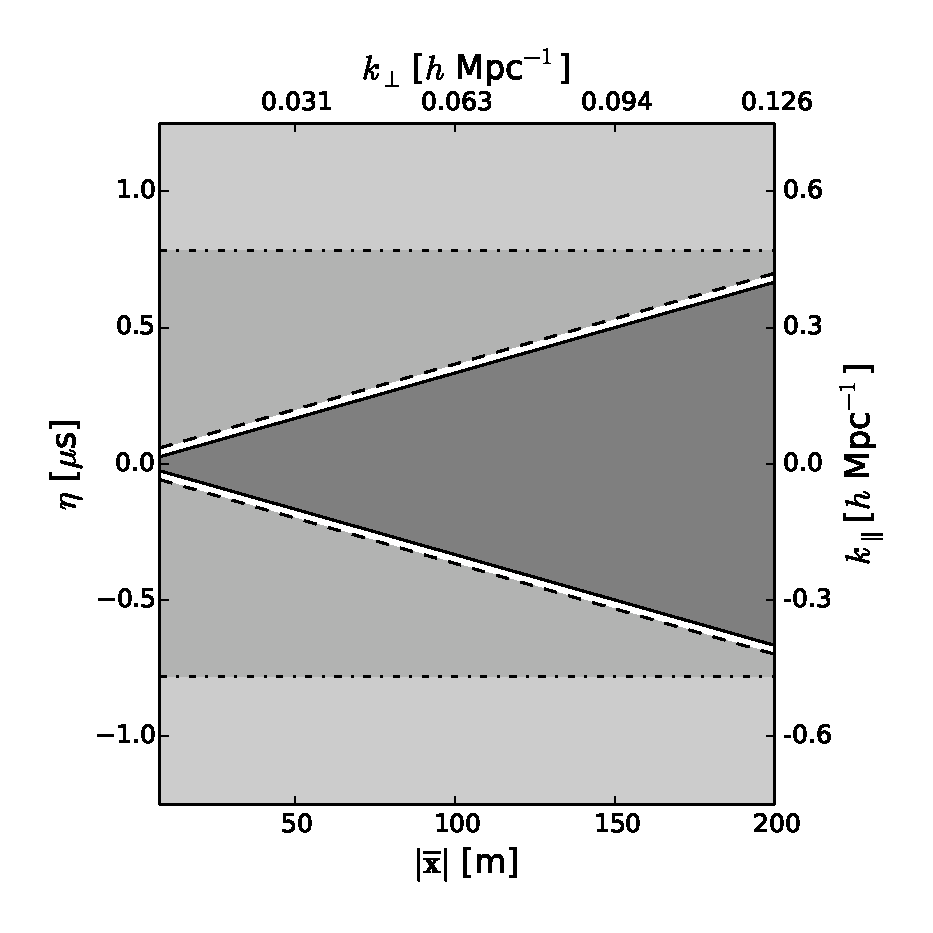
\includegraphics[width=\linewidth]{figures/v1_0/fourier_space_185.0_MHz_30.7_MHz.eps}
\caption{Fourier space in which delay (and power) spectra of EoR H{\sc i} signals are presented. The $x$--axis is denoted by $|\vec{b}|$ (antenna spacing) or $k_\perp$ (transverse wavenumber). The $y$--axis denoted by $\tau$ (delay) or $k_\parallel$ (line--of--sight wavenumber). Here, $k_\perp$ and $k_\parallel$ are obtained for a frequency of 185~MHz. The dark shaded region is referred to as the {\it foreground wedge} where smooth spectrum foregrounds reside. Its boundaries (solid lines), given by light travel time for corresponding antenna spacings, are referred to as horizon delay limits. Regions excluding the {\it wedge} and narrow extensions of the {\it wedge} (white unshaded strips) caused by convolution with the instrumental transfer function are expected to be relatively free of foreground contamination. Due to an undesirable grating pattern (dot--dashed lines) of the instrument used in this study, namely the MWA, we conservatively identify a restricted region of high EoR sensitivity (medium shade) and refer to it as the {\it EoR window} in this paper. \label{fig:fourier-space}}
\end{figure}

% The terms antenna spacing and baseline are synonymous in radio interferometry. The latter term is also used broadly to refer to the antenna pair system in a radio interferometer array. We use these terms interchangeably in this paper. 

For geometrical intuition, we restrict the orientation ($\theta_b$, measured anti-clockwise from East) of all baselines to lie in the range $-67\fdg 5 \leq \theta_b < 112\fdg 5$. Baselines oriented in the other half--plane measure conjugate visibilities with delays of equal magnitude but of opposite sign and hence are ignored in our analysis.

\section{Example Data}\label{sec:instrument}

\subsection{The Murchison Widefield Array (MWA)}

The MWA construction was completed in 2012 and, after commissioning, began its EoR observing program in 2013. In its final configuration the MWA is a 128--tile interferometer array capable of observing a 30.72~MHz instantaneous band anywhere in the range 80--300~MHz. Each tile is a phased array of 16 dipoles, each in the shape of a bow--tie. This yields a primary field of view $\gtrsim$~20\arcdeg~ wide and multiple secondary lobes. The array is arranged as a centrally condensed core of $\sim$~300~m --- there are many spacings in the range 5--50~m --- and a radial density that falls off as the inverse of the radius, with the longest baselines at 3~km \citep{bea12}. Here we focus on antenna spacings $|\vec{b}| \le 200$~m (spatial scales relevant to reionization) and a frequency range 170--200~MHz. The center frequency of 185~MHz corresponds to a redshift, $z\simeq 6.68$.

The MWA passband of width 30.72~MHz is divided coarsely into 24$\times$1.28~MHz sub--bands with each sub--band weighted by a digital filter. The coarse channel shape is obtained using a 8--tap polyphase filter bank (PFB) and a Kaiser window with parameter $\beta=5$. After correcting for the shape of these coarse channels, the fine channels (40~kHz width) at the edges of these sub--bands are flagged because they are known to be contaminated by aliasing at a low level. Any spectral flags, or other known weights constitutes $W_f(f)$ in equation~\ref{eqn:obsvis}. 

% The bandpass properties used in this paper are illustrated in Figure~\ref{fig:bandpass}. The MWA bandpass of width 30.72~MHz is divided coarsely into 24 1.28~MHz chunks (dashed lines connecting solid circles) with each chunk weighted by a digital filter. The coarse channel shape is obtained using a 8--tap polyphase filter bank (PFB) and a Kaiser window with parameter $\beta=5$. The bandpass correction ({\it plus} symbols connected by dotted lines) corrects for the shape of the coarse channels. After this correction, the channels at the edges of these chunks have been flagged (solid lines) because they are known to possibly be contaminated by aliasing at a low level. Any spectral flags, or other known weights constitutes $W_f(f)$ in equation~\ref{eqn:obsvis}. 

% \begin{figure}[htb]
% \centering
% 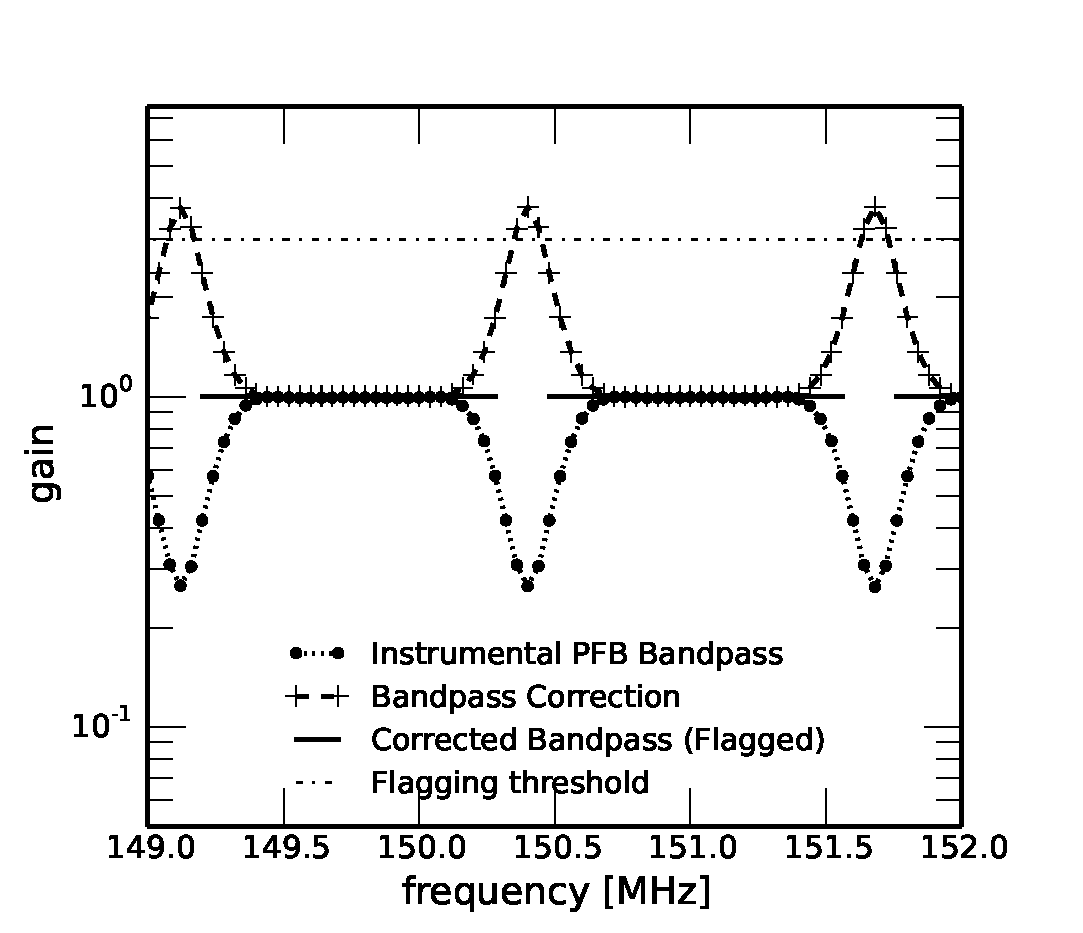
\includegraphics[width=\linewidth]{figures/v1_0/bandpass_properties.eps}
% \caption{Bandpass properties used in modeling and analysis of delay spectrum of MWA visibilities. The filled circles joined by dotted lines show the 8--tap PFB bandpass shapes obtained using a Kaiser window with parameter $\beta=5$. The bandpass correction factors applied are shown ({\it plus} symbols connected by dashed lines). The solid line shows the flagged (gaps) and gain--corrected bandpass shape. These shapes are repeated every 1.28~MHz for the entire bandwidth of 30.72~MHz centered around 185~MHz. \label{fig:bandpass}}
% \end{figure}

Thermal noise in simulated visibilities is estimated assuming a system temperature of $T_\textrm{sys}=95$~K per polarization for all frequency channels for all antenna pairs throughout the course of the observation. Estimation of $T_\textrm{sys}$ from MWA data is a subject of active investigation. In our work, we have chosen a $T_\textrm{sys}$ that matches the thermal noise observed in the data. % We take into account the increase in thermal uncertainty in frequency channels that results due to aforementioned bandpass correction. ({\bf Since the bandpass correction is digital, shouldn't the noise stay flat after bandpass correction? -- JDB: yes})

\subsection{Observation Parameters}\label{sec:obsparms}

The MWA targets two primary low-foreground fields for reionization observations. Here, we focus on the field at RA = 0h, Dec = $-30$\arcdeg. The MWA tracks a patch of sky through antenna beams formed and steered electronically by controlling delay settings of the dipoles in an MWA tile. The pointing system is capable of steering to points on a regular $\sim$7\arcdeg~ grid. During observations we allow the sky to drift across the nearest available pointing, shifting between grid points as necessary (once in $\sim 30$~minutes). This process is repeated throughout the course of the observation $\approx 4.86$~hours. Figure~\ref{fig:pointings} illustrates how the apparent pointing oscillates around the desired pointing direction. 

The observations shown here were undertaken on Aug~23, 2013. % Data set from this day has been chosen as a reference for comparison within the MWA EoR collaboration because this is one of the days featuring a low number of known system errors from among a long stretch of stable observing.  
We have chosen two, 112 second long sections from this night for detailed study. These were chosen to provide a selection of possible foreground and instrumental conditions. As an example of a nominal observing setup we choose a zenith pointing; as an example of poor foreground conditions, we choose a pointing when the field is $\sim 2$~hours from zenith. This pointing has a significantly higher secondary lobe structure and is observed when the bright galactic center is well above the horizon. 

The {\it local sidereal time} (LST) at these two snapshots are shown in Figure~\ref{fig:pointings} as vertical lines at $-1.92$~hours (i.e., 22.08~hours) and 0.09~hours which are hereafter denoted as {\it off--zenith} and {\it zenith} pointings, respectively. %These pointings (phased array power--patterns) are centered at RA = 4\fdg 387, Dec = -29\fdg 86 and RA = -28\fdg 8, Dec = -26\fdg 701, whereas the visibilities themselves are phased to zenith corresponding to RA = -28\fdg 8, Dec = -26\fdg 701, and RA = 1\fdg 35, Dec = -26\fdg 701 respectively.   

\begin{figure}[htb]
\centering
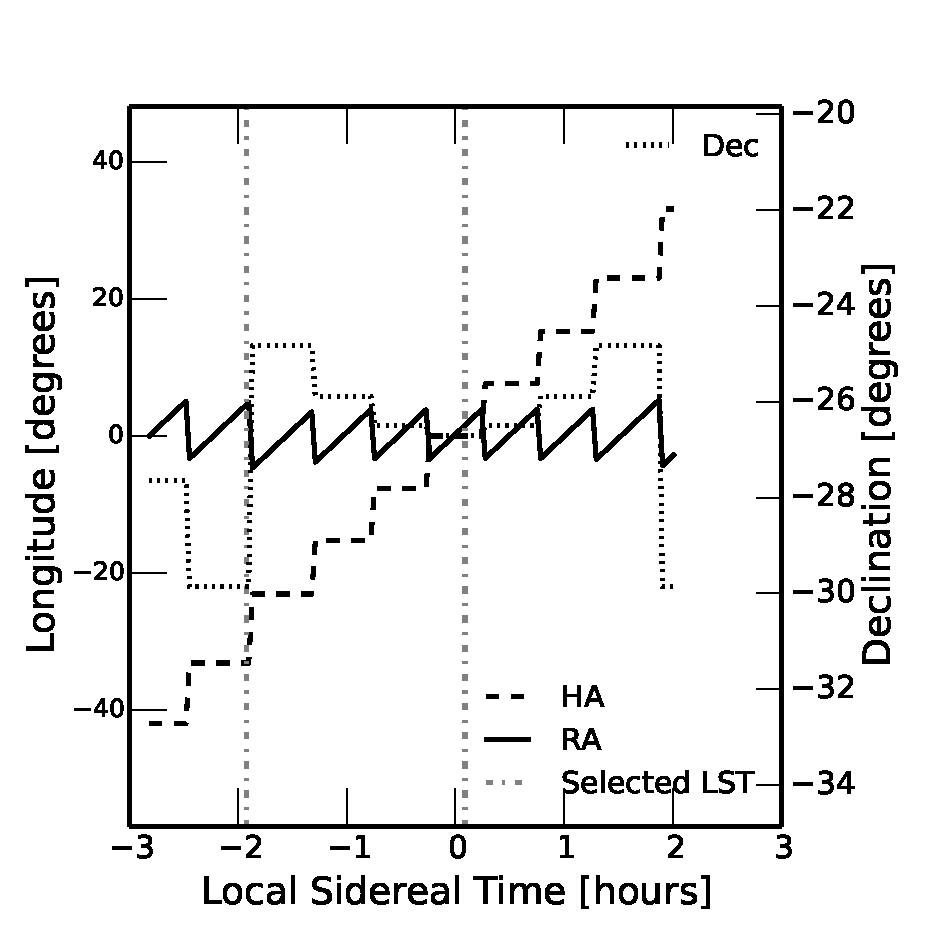
\includegraphics[width=\linewidth]{figures/v1_0/custom_pointings.eps}
\caption{MWA tile beam pointing directions during the course of the observation. The $x$--axis refers to the {\it local sidereal time} (LST). The axis on the left refers to longitudes, namely, Right Ascension (RA) and Hour Angle (HA). Negative values of RA, HA, and LST are to be interpreted as having been wrapped around by 360\arcdeg~ or 24 hours. The axis on the right refers to the declination of the pointing direction. The RA, HA, and declination are plotted with solid, dashed and dotted lines respectively. The sky is allowed to drift for $\sim 30$~mins before the beamformer delay settings change in a discrete step to center the beam around RA = 0h, Dec = $-30$\arcdeg. Dot--dashed vertical lines show the LST of {\it off-zenith} and {\it zenith} pointings used in our study. \label{fig:pointings}}
\end{figure}

\subsection{Initial Data Processing}\label{sec:data-analysis}

The data are flagged\footnote{\url{http://sourceforge.net/p/aoflagger}} for interference \citep{off12,off10}, removing 3\% of the data and averaged in time  and frequency from the raw 0.5~s, 40~kHz to 2s, 80~kHz. These data are then calibrated to a simulation of the sky containing 2420 point--like objects selected from the MWA Commissioning Survey (MWACS; Hurley-Walker et al. 2014, submitted). % MWACS was compiled using observations taken with subsets of the array during the final buildout and commissioning;
It has a flux density limit of 25~mJy and a declination range of -12\arcdeg~ to -40\arcdeg~ evenly covering the field of view of the observations reported here. The objects used in calibration are selected to lie inside the 5\% contour of the primary lobe of the tile power--pattern. The calibration algorithm -- based on forward modeling software by \citet{sul12} -- computes complex gain solutions per channel per antenna averaged to two minute intervals. The solutions are fairly low signal--to--noise so we iteratively project along the antenna and frequency dimensions to capture the relatively independent passband and antenna--to--antenna variation. First, we average the channel gains over all antennas to obtain a high signal--to--noise measurement of the bandpass. After applying this single passband, we do a second round of calibration and fit second and first order polynomials for amplitude and phase respectively for each antenna. This flattens any residual variation in bandpass and removes small phase slopes due to variations in cable delay. Finally, we fit for an additional phase known to be caused by reflections in a few 150~m length cables. %possibly could add elaboration, if I knew exactly which version of the cal was done here. doesn't really matter

\subsection{Deconvolved Delay Spectrum}\label{sec:data-delay-spectrum}

We obtain the delay spectrum of these calibrated visibilities taking the delay transform of each baseline's spectrum (equation~\ref{eqn:delay-transform}) choosing $W'_f(f)$ to be a {\it Blackman--Harris} window function. The spectrum is multiplied by the additional weight of the flagged channels which occur rarely for interference and regularly every 1.28~MHz where the edges of coarse channels are known to have a small aliasing effect. In delay--space, these weights translate into a convolution by a grated point spread function (PSF) with gratings at multiples of $\tau=0.78\,\mu$s. We deconvolve this PSF using a one dimensional CLEAN algorithm \citep{tay99} as described for the delay axis by \citet{par09,par12}. The CLEAN procedure iteratively finds and subtracts peak values convolved by the Fourier transform of the weights. We limit the selection of peaks to modes inside the horizon delay limit, corresponding to smooth spectrum objects in the visible sky hemisphere.

In subsequent sections, we plot the amplitude of the delay spectrum, $|V_{b\tau}(\vec{b},\tau)|$, sorted by baseline length, $|\vec{b}|$. Note that visibilities from different baselines have not been averaged together in this analysis. 

We show results of delay spectrum from MWA data after deconvolution along the delay axis in Figure~\ref{fig:fhd_data}. The principle feature is the {\it foreground wedge}, whose boundaries, marked by white lines, increase linearly with light travel time corresponding to baseline length. Note that the wedge is not filled out uniformly. Each baseline has a different orientation and resulting response to different objects in the sky. It is this variation that we will explore below. 

The {\it off--zenith} pointing has emission notably higher than in the {\it zenith} pointing inside the {\it foreground wedge}. This is shown later to be due to response of the array to the bright Galactic center and Galactic plane in the westward sky. Consequently, the contamination into the {\it EoR window} is also higher, especially on short antenna spacings. Emission in the {\it zenith} pointing is more centrally concentrated due to phasing of power--pattern to the zenith, whereas the {\it off--zenith} pointing has a power--pattern phased eastward of zenith but is also responsive to emission from angles far away from zenith. 

\begin{figure}[htb]
\centering
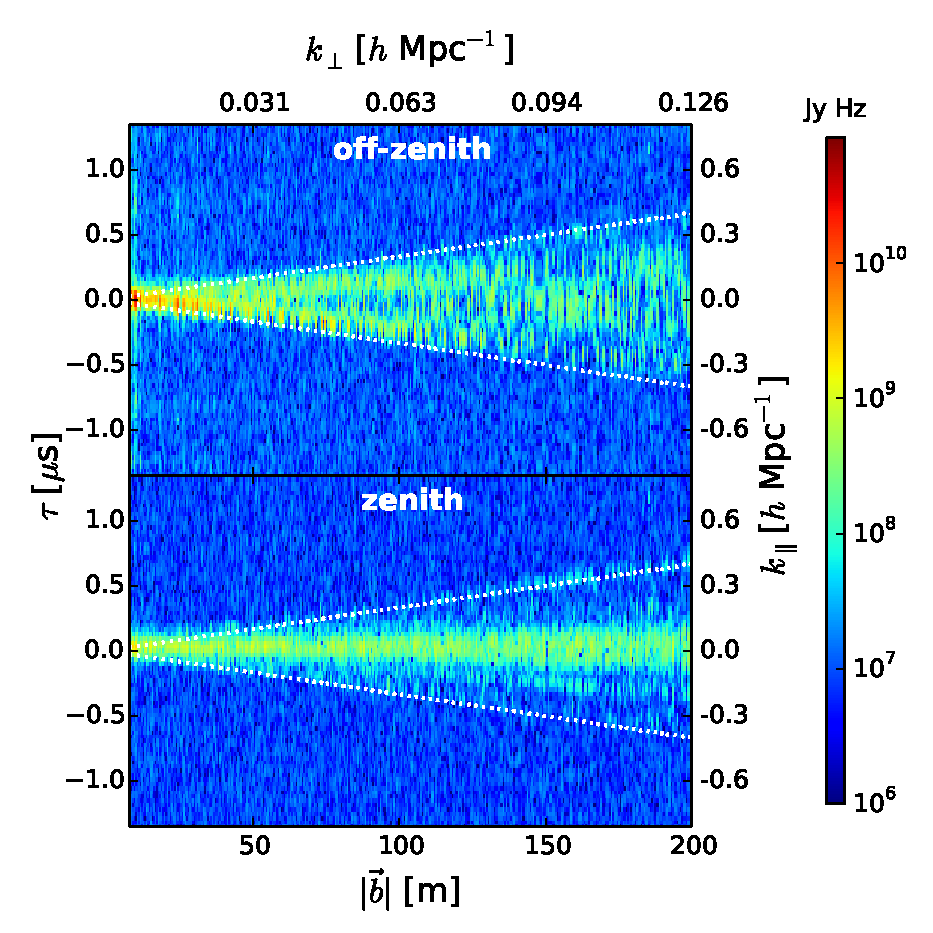
\includegraphics[width=\linewidth]{figures/v1_0/multi_baseline_fhd_delay_spectrum_snapshots.eps}
\caption{Delay spectra of two observations of the EoR field (RA = 0h, Dec = $-30$\arcdeg) at an {\it off--zenith} pointing (top) when tiles have significant secondary lobes in the direction of the Galactic center and a {\it zenith} pointing (bottom) where secondary lobes are minimal and the Galaxy has set. For reference, the $k$--space equivalent of $\tau$ and $|\vec{b}|$, namely, $k_\parallel$ and $k_\perp$ are shown at the axes on the right and top respectively. White lines mark the boundaries of {\it foreground wedge} determined by light travel time across each baseline. Smooth spectrum objects predominantly reside in this {\it foreground wedge}. The logarithmic color scale (shown at the right) is common to both panels. \label{fig:fhd_data}}
\end{figure}

% Despite delay deconvolution, we still see leakage beyond the cleaned regions indicating the inability of the deconvolution algorithm to fit the measurements perfectly, dominant at short antenna spacings where the number of delay modes within the horizon is lesser. This is because the maximum delay envelope (boundary of the wedge) consists of mixed emission from large portions of the sky into a narrow range of delays and the deconvolution algorithm does not have sufficient support in delay space to fit the delay spectrum. However, we wish to emphasize that the purpose of deconvolution is to rid the delay spectra of instrumental artifacts to the best extent possible in order to see the underlying signatures of foreground emission. It is not our intention in this paper to use the deconvolution as a foreground removal tool. 

\section{Simulations}\label{sec:modeling}

We describe the instrumental and foreground models we use in our simulations. 

\subsection{Instrument Model}\label{sec:instrument_model}

The instrument model consists primarily of the tile beam power--pattern, $A(\hat{s},f)$ (see equation~\ref{eqn:obsvis}). It is modeled as a mutually--coupled 4--by--4 dipole array with the overall power--pattern of each individual dipole calculated via finite element electromagnetic simulation \citep{sut14}. To speed up simulations, we find that a phased array of isotropic radiators at a height of 0.3~m above an infinite ground plane provides a very good approximation to the full simulation, hence we use the idealized dipoles. We also assume that each individual dipole signal has random delay fluctuations of rms 0.05~ns, a number in line with the known repeatability and stability level of the analog signal chain \citep{bow07b}. Besides having the effect of adding a time--dependent uncertainty in the power pattern, these random delay fluctuations reduce the coherence in the phased addition of dipole signals resulting in deviations from predicted models of the power--pattern, most prominently at its nulls. The power--patterns so obtained are shown in Figure~\ref{fig:power_pattern} for the pointings chosen in our study.

\begin{figure}[htb]
\centering
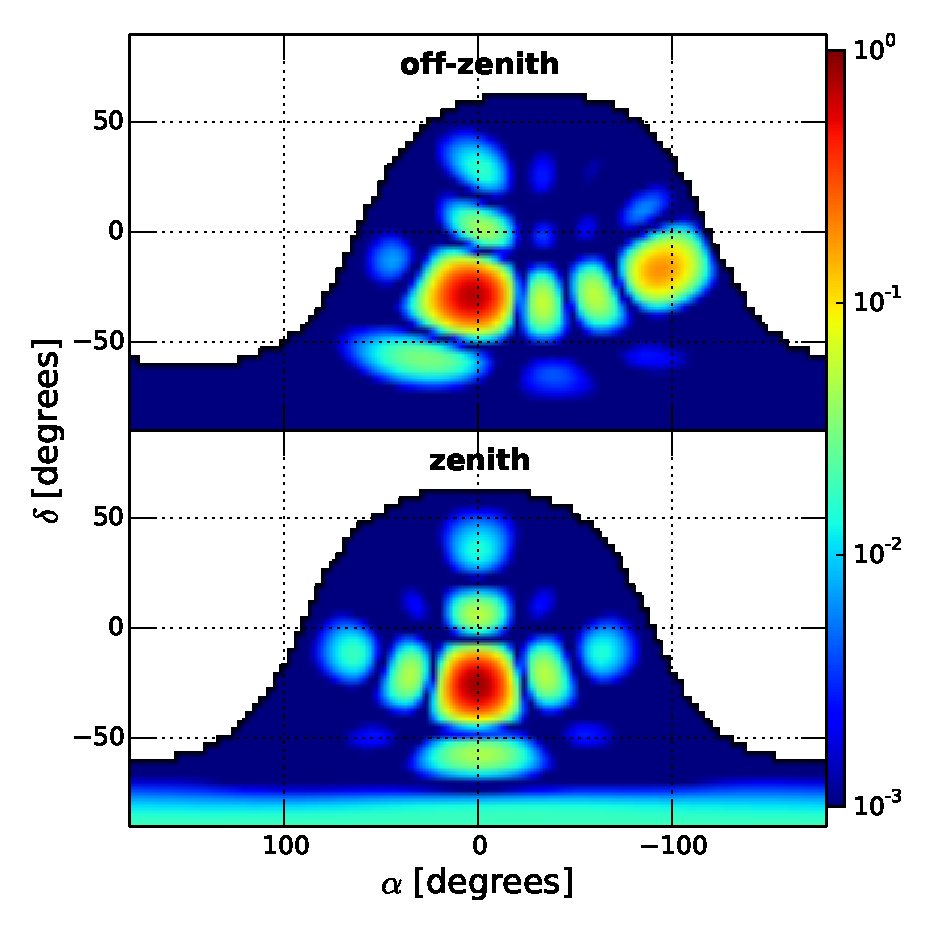
\includegraphics[width=\linewidth]{figures/v1_0/delta_array_powerpattern_0.3m_ground_custom.eps}
\caption{Models of MWA tile power--pattern for {\it off--zenith} (top) and {\it zenith} pointings (bottom) at 185~MHz. An MWA tile is modeled as a 4$\times$4 array of isotropic radiators placed 0.3~m above an infinite ground plane. Random fluctuations of rms 0.05~ns have been added to delay corrections during the phased addition of voltages from these isotropic radiators. The logarithmic color scale (shown on the right) is common to both panels. \label{fig:power_pattern}}
\end{figure}

\subsection{Foreground Model}\label{sec:foreground}

The MWA has a very wide field of view ($\gtrsim 20$\arcdeg~ at 185~MHz) and has non--negligible response all the way to the horizon. As already noted, foreground objects fill the {\it foreground wedge} with an amplitude which depends on the tile power gain in that direction, with objects at the horizon being closest to the boundaries of the {\it wedge}. 

The degree to which these objects leak power into spectral line of sight modes in the {\it EoR window} will be shown to depend primarily on the brightness of foregrounds near the boundaries of the {\it foreground wedge}. Thus, it is important to consider an all--sky model for foreground objects in evaluating the features seen in the power spectrum instead of restricting only to the primary field of view. 

% JDB: I don't think we need this here. %% \citet{bea13} estimated the sensitivity of the MWA to EoR H{\sc i} power spectrum detection taking into account thermal noise effects in the {\it EoR window}. \citet{thy13} estimated the sensitivity taking into account the spillover from foreground contamination from unsubtracted extragalactic compact objects in the {\it EoR window} besides thermal noise. In this paper, we include the diffuse Galactic emission for enhancing our understanding of foreground signatures in the power spectrum. 

We use an all--sky foreground emission model that includes both diffuse and bright compact components.  

\subsubsection{Diffuse Foreground Model}\label{sec:DSM}

For the diffuse component, we use an all--sky radio foreground model \citep{deo08} to estimate the emission at 185~MHz. At this frequency, since this map is predominantly based on the 408~MHz all--sky map of \citet{has82} which has an angular resolution of 0\fdg 85, we smoothed the 185~MHz map to the same resolution. However, to avoid any artifacts from sampling this map, we sample it at $\approx 27$\arcmin~intervals. We model the diffuse foreground spectra with a single spectral index at each pixel in the map, found by comparing model maps at 170~MHz and 200~MHz.

A low resolution version of the diffuse foreground model used is shown in Figure~\ref{fig:DSM}. Contours of the MWA tile power--pattern shown in Figure~\ref{fig:power_pattern} are also overlaid. Of notable significance in the {\it off--zenith} pointing is the presence of a portion of the Galactic plane and the bright Galactic center in the westward sky, where the MWA tile power gain is significant ($\gtrsim 12$\%). In the {\it zenith} pointing, the Galactic plane has set and the power--pattern in that direction is at least 16 times smaller. 

\begin{figure}[htb]
\centering
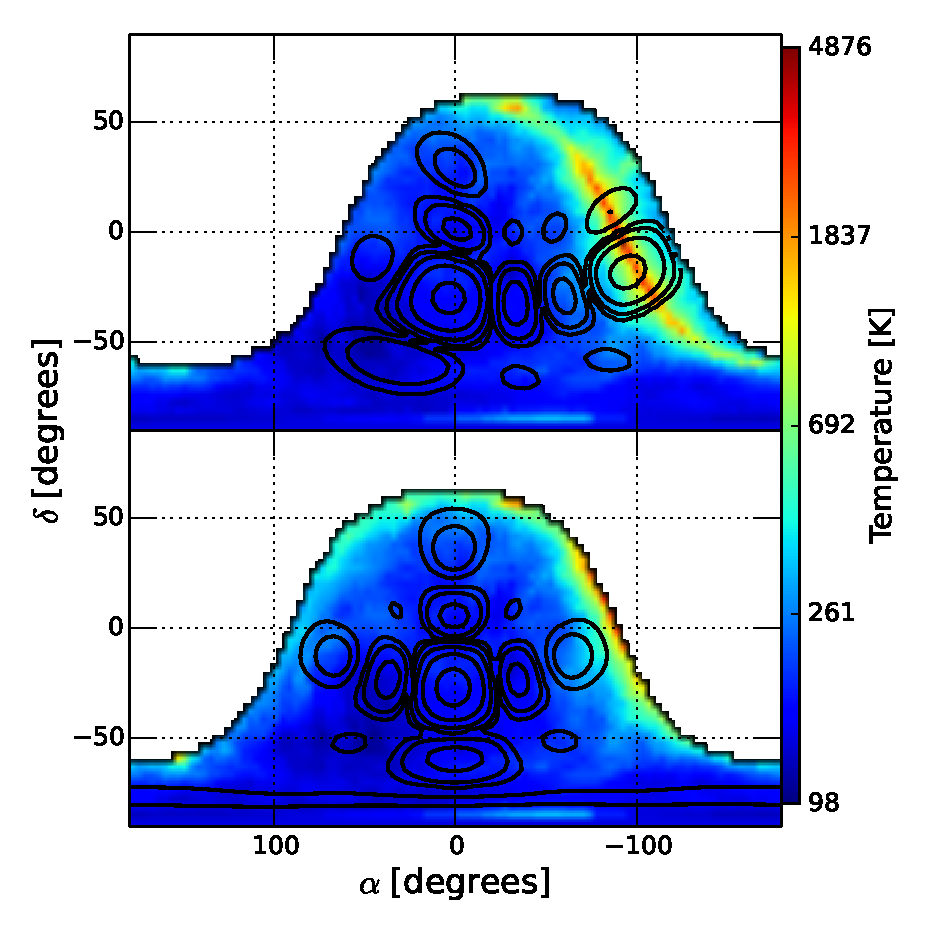
\includegraphics[width=\linewidth]{figures/v1_0/dsm.eps}
\caption{Sky brightness temperature of the diffuse foreground model at 185~MHz visible during {\it off--zenith} (top) and {\it zenith} (bottom) pointings. The color scale on the right is logarithmic and is common to both panels. Contours of power--pattern shown in Figure~\ref{fig:power_pattern} are overlaid. The contour levels shown are 0.00195, 0.00781, 0.0312, 0.125, and 0.5. The Galactic center and a portion of the Galactic plane are prominently visible during the {\it off--zenith} pointing and the MWA tile power gain is significant ($\gtrsim 12$\%) in that direction. In contrast, emission from the Galactic plane in {\it zenith} pointing is significantly lesser. \label{fig:DSM}}
\end{figure}

\subsubsection{Compact Foreground Model}\label{sec:CSM}

The model described in the preceding section is primarily a model of the diffuse foreground sky. While it contains faint compact emission blended in with the diffuse emission, it is known to be devoid of bright point sources \citep{deo08}. In order to supplement it with missing bright compact emission, we use classical radio source confusion estimates to determine the nominal flux density threshold and include point sources brighter than this threshold. It may be noted that slightly different criteria are in common use in radio astronomy to estimate radio source confusion \citep[see Appendix of][and references therein]{thy13}. For an angular resolution of 0\fdg 85, using a conservative `$S_\textrm{c}=5\sigma_\textrm{c}$' criterion, we determine the flux density threshold to be $\approx 10$~Jy. Other liberal criteria that yield a lower threshold carry a greater risk of double--counting point sources which might be already blended in with the diffuse sky model. 

We use a combination of the NRAO VLA Sky Survey \citep[NVSS;][]{con98} at 1.4~GHz and the Sydney University Molonglo Sky Survey \citep[SUMSS;][]{boc99,mau03} at 843~MHz to provide our point source catalog due to their complementary survey footprints covering the entire sky, and matched flux density sensitivity and angular resolution. The SUMSS catalog covers the sky with declination $\delta < -30$\arcdeg~ with a limiting peak brightness of 6--10~mJy/beam and an angular resolution of $\sim 45$\arcsec. The NVSS covers the sky with $\delta > -40$\arcdeg~ with a similar angular resolution and a limiting flux density of $\approx 2.5$~mJy for point sources. 

From the SUMSS catalog, we select point sources whose deconvolved major axes are equal to 0\arcsec. From the NVSS catalog, we excluded objects that overlap with those in the SUMSS survey footprint. Point sources from NVSS were selected if the convolved major axes were not greater than $\approx 47$\arcsec, which is almost equal to the angular resolution of the survey. Using a mean spectral index of $\langle\alpha_\textrm{sp}\rangle=-0.83$ (flux density, $S(f)\propto f^{\alpha_\textrm{sp}}$) obtained by \citet{mau03} for both NVSS and SUMSS catalog objects, we calculate the corresponding flux densities at 185~MHz, $S_{185}$. From this subset, we choose point sources with $S_{185}\geq 10$~Jy. The selection of such bright point sources is not affected by minor differences in flux density sensitivity of the two surveys. We verified that our selection criteria ensure a similar areal density of objects in the two surveys. 

Based on these criteria, we selected 133 objects from the SUMSS catalog and 336 objects from the NVSS catalog. Together with the diffuse foreground model, we obtain an all--sky foreground model consisting of both compact and diffuse emission. Figure~\ref{fig:CSM} shows the compact foreground emission model used in our study whose with contours of the power pattern overlaid. The flux densities of the point sources are indicated by the color scale. 

\begin{figure}[htb]
\centering
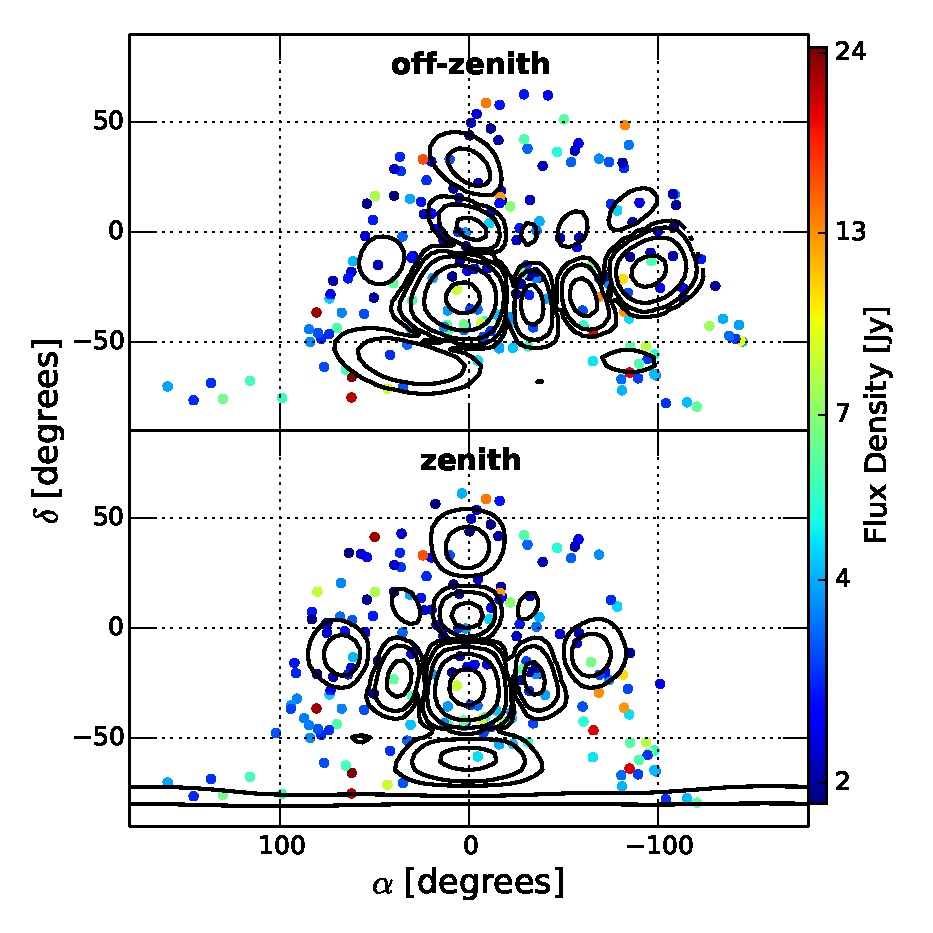
\includegraphics[width=\linewidth]{figures/v1_0/csm.eps}
\caption{Flux densities of bright point sources at 185~MHz visible during {\it off--zenith} (top) and {\it zenith} (bottom) pointings. The color scale on the right is logarithmic and is common to both panels and corresponds to the color--coded filled circles. Contours of power--pattern shown in Figure~\ref{fig:power_pattern} are overlaid. The contour levels shown are 0.001953125, 0.0078125, 0.03125, 0.125, and 0.5. \label{fig:CSM}}
\end{figure}

It is worth emphasizing that the ideal foreground model is one with an angular resolution finer than that of the instrument that covers the whole sky at the observing frequency, a point we will revisit later. For this study, we note that our conclusions are not significantly affected despite minor differences in the thresholds from different radio source confusion estimates.

\subsection{Comparison with Data}\label{sec:data-vs-model}

With the aforementioned all--sky foreground model, and instrumental and observational parameters, we simulate visibilities using equation~\ref{eqn:obsvis}. Figure~\ref{fig:sim_data} shows the amplitude of the delay spectrum from {\it off--zenith} and {\it zenith} pointings. Notice the qualitative agreement of amplitude and structure with those obtained from data shown in Figure~\ref{fig:fhd_data}. The Galactic center and the Galactic plane visible in the {\it off--zenith} pointing make it appear brighter in the {\it foreground wedge}. 

\begin{figure}[htb]
\centering
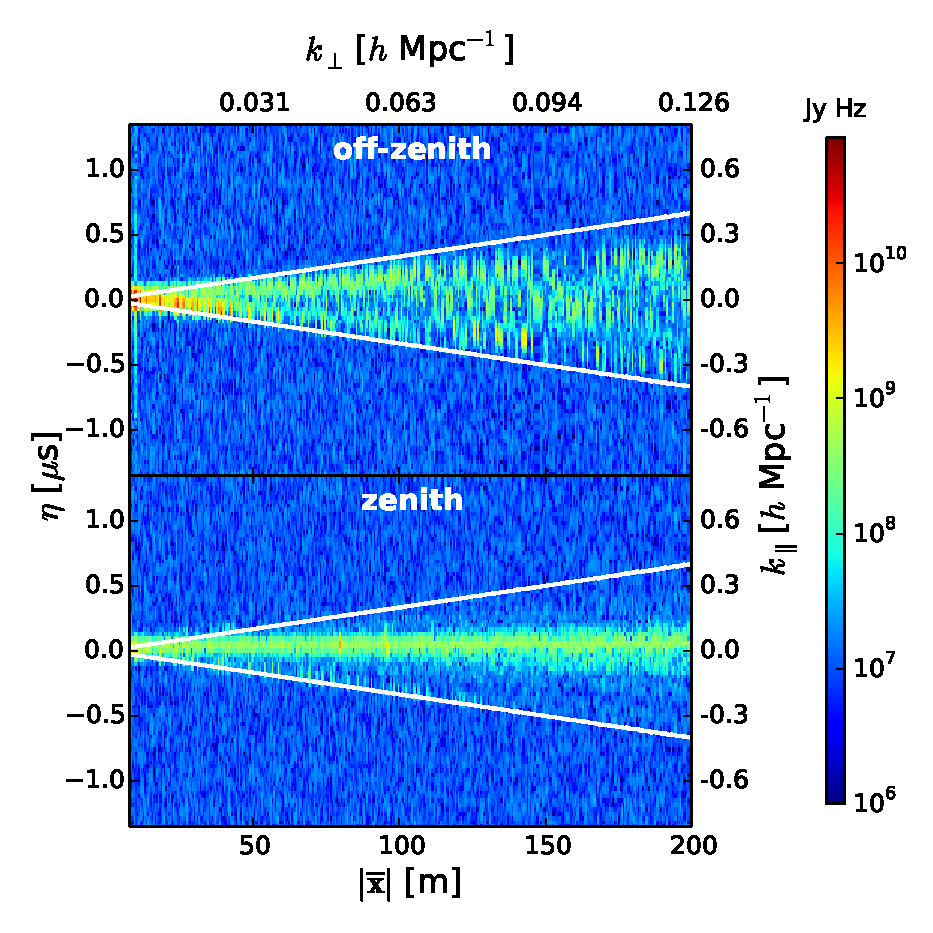
\includegraphics[width=\linewidth]{figures/v1_0/multi_baseline_sim_delay_spectrum_snapshots.eps}
\caption{Same as Figure~\ref{fig:fhd_data}, but generated from simulated visibilities using the model described in \S\ref{sec:modeling}. Note the similarity between the broad features to those in Figure~\ref{fig:fhd_data}. \label{fig:sim_data}}
\end{figure}

In order to make a quantitative comparison of delay spectra obtained with MWA data and our simulations, we consider the uncertainty in the assumed spectral index of our foreground model. Our foreground models are derived from other higher frequency catalogs and sky maps. The inherent spread in spectral index increases the uncertainty while predicting fluxes at the observing frequency. Using simple error propagation, the fractional error in the delay spectrum caused by the spread in spectral index is $\sim \ln(f_\textrm{orig}/f)\,\Delta\alpha_\textrm{sp}$, where, $f_\textrm{orig}$ is the original frequency at which the catalog or map was created, $f=185$~MHz is the MWA observing frequency, and $\Delta\alpha_\textrm{sp}$ is the spread (HWHM) in spectral index. From \citet{mau03}, we assume $\Delta\alpha_\textrm{sp} \approx 0.35$ for point sources from NVSS and SUMSS catalogs. Although the model of \citet{deo08} yields a spectral index per direction on the sky, we could assume similar uncertainties exist in spectral indices of our diffuse sky model as well, which is predominantly derived from the 408~MHz map of \citet{has82}. Thus, fractional errors in delay spectrum from compact and diffuse components are $\sim$70\% and $\sim$30\% respectively. 

In addition to intrinsic model uncertainty, delay spectra from simulations and data each have fluctuations due to thermal noise in the delay spectrum with rms $\sim$ 1.4$\times 10^7$~Jy~Hz. We estimate the ratio of delay spectra from data and simulations as $\rho = |V^\textrm{D}_{b\tau}(\vec{b},\tau)|\,/\,|V^\textrm{S}_{b\tau}(\vec{b},\tau)|$, where superscripts D and S denote data and simulation, respectively. % Using the aforementioned uncertainties added in quadrature, we estimate the approximate expected uncertainty in $\log_{10}\rho$ and denote it by $\Delta\,\log_{10}\rho$. 

Figure~\ref{fig:data-sim-ratio} shows normalized histograms of the distribution of $\log_{10}\rho$ for the {\it off--zenith} (top panel) and {\it zenith} (bottom panel) pointings respectively inside the {\it foreground wedge}. The median absolute deviation from these distributions corresponds to $\sim$~90\% fractional difference between data and modeling on average in either case. This is in line with expectations when the aforementioned uncertainty in foreground models, thermal noise fluctuations in measurements, and uncertainties in antenna power pattern due to random delay fluctuations are taken into account. Currently, we are significantly limited by the unavailability of all--sky foreground models at the observing frequency of 185~MHz. 

\begin{figure}[htb]
\centering
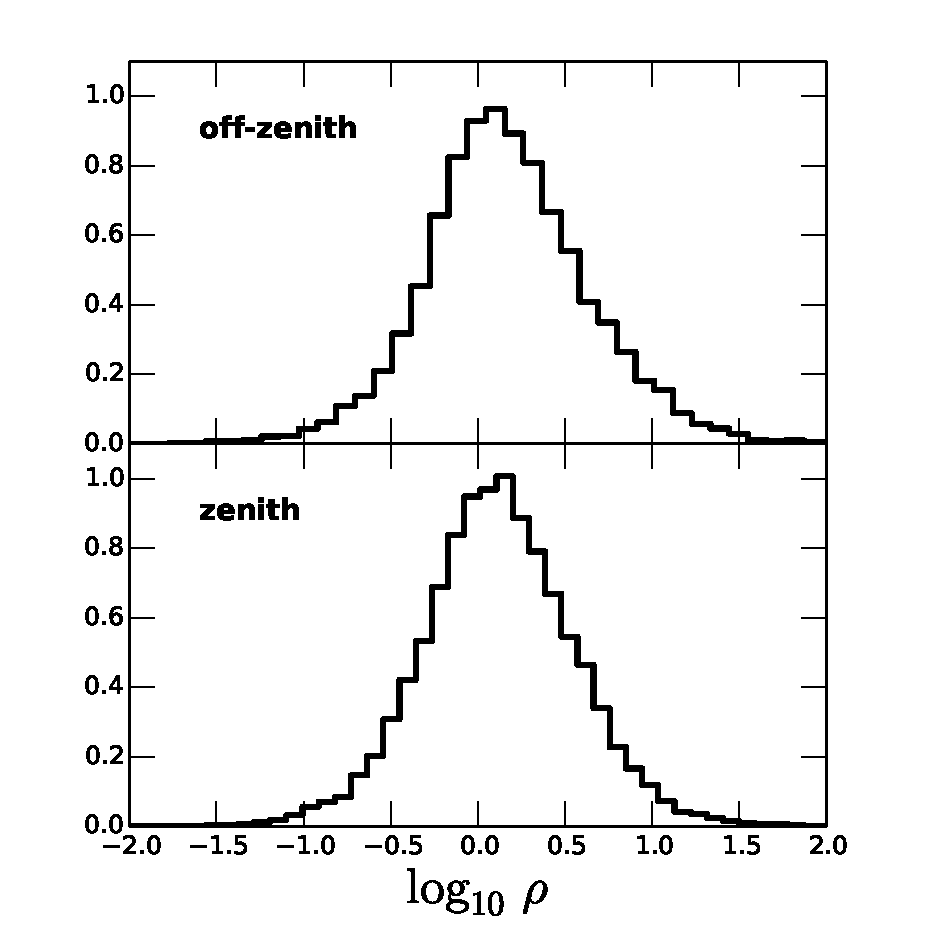
\includegraphics[width=\linewidth]{figures/v1_0/delta_array_histogram_wedge_sim_data_log_ratio_0.3m_ground_custom_gaussian_FG_model_asm_all_sky_nside_64_Tsys_95.0K_185.0_MHz_30.7_MHz_bhw2.0.eps}
\caption{Normalized histograms of logarithm of ratios of observed to simulated visibilities restricted to the {\it foreground wedge} -- i.e., within the white lines of Figure \ref{fig:sim_data} -- for the {\it off--zenith} (top) and {\it zenith} (bottom) pointings. Median absolute deviation of $\log_{10}\rho$ is $\sim 0.28$ in both cases indicating a fractional difference of $\sim 90$\%. A value of zero indicates perfect agreement ($\rho=1$). \label{fig:data-sim-ratio}}
\end{figure}

These uncertainties are presented to confirm the qualitative agreement already seen between Figures~\ref{fig:fhd_data} and \ref{fig:sim_data}. These uncertainty estimates are conservative. A full treatment of all uncertainties and deviations from ideal behavior such as frequency dependent errors in tile power--pattern \citep{ber14}, calibration \citep{dat10}, data corruption due to interference, anisoplanatic wide--field imaging and ionospheric effects \citep{int09} will bring the simulations much closer in agreement with observations, but is beyond the scope of this paper. Our primary objective is to explore in detail the foreground signatures embedded in the {\it foreground wedge}.

\section{Results}\label{sec:delay-spectrum-analysis}

Having established that the simulation matches the data to the level of expected uncertainties, we proceed to examine in further detail the key signatures seen in simulated delay spectra. A number of factors are responsible for the characteristics noted in the delay spectra obtained from data and through simulations. We address these factors below: 

\begin{itemize}

\item {\it Sky Model}: Our model of the sky consists of compact and diffuse emission on diverse spatial scales as shown in Figures~\ref{fig:DSM} and \ref{fig:CSM}. It also consists of localized regions of strong emission such as the Galactic plane and Galactic center. The resulting sky emission is anisotropic. In fact, the patch of sky for MWA observations is chosen from regions of low foreground emission. We will investigate the signatures of each component and their potential impact on {\it EoR window} contamination.

\item {\it Baseline Orientation}: Since the spatial structure of our foreground model is not expected to be isotropic, we divide our antenna spacings by their orientation, $\theta_\textrm{b}$. We use the following bins: $-67\fdg 5\le \theta_\textrm{b} < -22\fdg 5$, $-22\fdg 5\le \theta_\textrm{b} < 22\fdg 5$, $22\fdg 5\le \theta_\textrm{b} < 67\fdg 5$, and $67\fdg 5\le \theta_\textrm{b} < 112\fdg 5$. The bin centers are oriented towards South--East, East, North--East, and North respectively. Since delays depend on $\theta_\textrm{b}$, binning by $\theta_\textrm{b}$ allows us to match delay spectrum features to different sky directions.

\item {\it Tile Pointing and Power--Pattern}: Since the MWA tiles are steered electronically, the power--pattern of the tile changes in any observing mode that tracks the object. In our study, we take into account the effect of the changing tile power--pattern on the delay spectrum (Figure~\ref{fig:power_pattern}). The LST of our data ranges from $\sim$~21 hours through $\sim$~2 hours, and for our analysis we chose the {\it off--zenith} and {\it zenith} pointings shown in Figure~\ref{fig:pointings}. We will show the secondary lobe structures in the tile power--pattern are tied to the foreground signatures in Fourier space. 

% \item {\it Instrumental Passband}: The instrumental passband characteristics have a direct effect on the delay transform owing to the Fourier relationship between the two. Due to excision of aliased edge channels repeated in each coarse channel of our passband, we observed repeated patterns of the {\it foreground wedge} in the delay spectra. As already mentioned earlier, we have used a deconvolution algorithm ({\it CLEAN}) to rid the delay spectra of band shape effects. Since this paper focuses on studying the effects of foreground on the delay spectra, we do not pursue the characterization of artifacts from the band shape and imperfections in {\it CLEAN} deconvolution.

\end{itemize}

In subsequent sections, we provide a detailed explanation of our results as a combination of factors noted above. Note that numerous features may overlap at different degrees of significance depending on combinations of parameters. We assign the features to their predominant causes. Secondly, we have used noiseless cases to clearly illustrate the observed foreground signatures. With the addition of noise in the visibilities which is subject to observing time, some of the weaker features may not be as prominently visible. Since the foreground signatures are far too numerous and they reside in a vast volume of parameter space such as antenna spacing length and orientation, power--pattern, patch of sky under observation, and instrumental configuration, we highlight only some examples of the most notable features observed in the delay spectra of foreground emission.

\subsection{Diffuse Foreground Signatures}\label{sec:diffuse}

Figure~\ref{fig:noiseless-dsm-delay-spectrum} shows the amplitude of delay spectrum, $|V_{b\tau}(\vec{b},\tau)|$, simulated with only the diffuse foreground model. The top and bottom panels correspond to {\it off--zenith} and {\it zenith} pointings, respectively. 

\begin{figure}[htb]
\centering
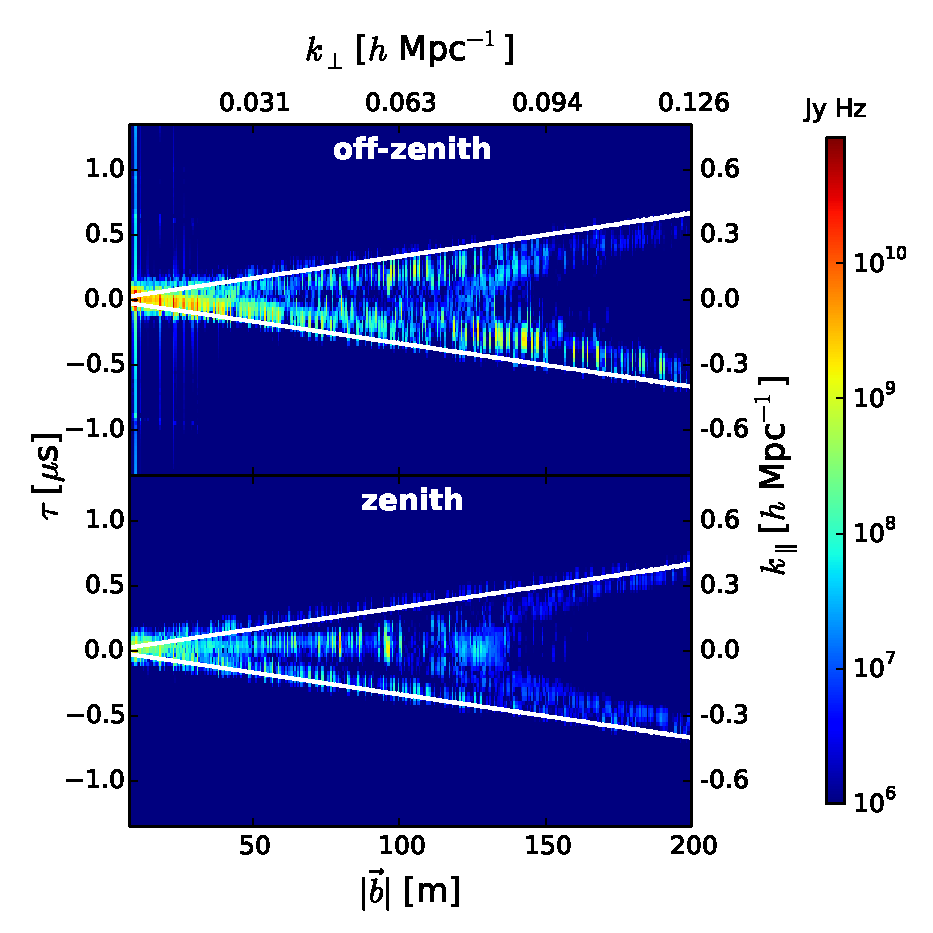
\includegraphics[width=\linewidth]{figures/v1_0/delta_array_multi_baseline_CLEAN_noiseless_visibilities_0.3m_ground_custom_gaussian_FG_model_dsm_all_sky_nside_64_Tsys_95.0K_185.0_MHz_30.7_MHz_bhw2.0.eps}
\caption{Simulated delay spectrum amplitudes $|V_{b\tau}(\vec{b},\tau)|$ (in units of Jy~Hz) for {\it off--zenith} (top) and {\it zenith} (bottom) pointings for the diffuse foreground model without any thermal noise. White lines mark the boundaries of the {\it foreground wedge} determined by the horizon delay limit and antenna spacing. The axes and color scale are identical to those in Figures~\ref{fig:fhd_data} and \ref{fig:sim_data}. In the {\it zenith} pointing, delay spectrum from diffuse emission has a {\it two--pronged fork}--shaped structure and is present even at wide antenna spacings. \label{fig:noiseless-dsm-delay-spectrum}}
\end{figure}

Here we examine in detail some examples of interesting features observed with the diffuse foreground model.

\subsubsection{Galactic Center on Eastward Antenna Spacings}\label{sec:GC-east}

The most prominent signature seen in the {\it off--zenith} pointing (top panel of Figure~\ref{fig:noiseless-dsm-delay-spectrum}) is due to the bright Galactic center situated on the western horizon co--located with one of the bright secondary lobes of the power--pattern. It appears as a bright branch in the delay spectrum near the negative delay horizon delay limit. This feature is strongest at short antenna spacings and fades with increasing antenna spacing. The signature is absent in the {\it zenith} pointing (bottom panel, Figure~\ref{fig:noiseless-dsm-delay-spectrum}) because the Galactic center is below the horizon. 

\subsubsection{Diffuse Emission Delay Spectra}\label{sec:diffuse-features}

Figure~\ref{fig:noiseless-dsm-delay-spectrum} also demonstrates diffuse emission from within the primary field of view manifests in the {\it off--zenith} pointing as a branch at the top of the wedge, and at zero delay in the {\it zenith} pointing. The former is seen at positive delays because the primary lobe of the power--pattern is centered eastward of zenith, whereas in the latter it is centered at zenith. As we see from Equation \ref{eqn:obsvis}, each baseline measures a single spatial mode on the sky with an angular size scale inversely proportional to the length of the baseline projected in the direction of the emission. Thus, in the {\it zenith} pointing, the signature of the smooth sky model, the horizontal line at zero delay, fades away on antenna spacings $|\vec{b}| \gtrsim 125$~m because the sky model is devoid of spatial structures on scales $\lesssim$~0\fdg 75. In the off-zenith pointing, we see power out to much longer baselines which is described below.

\subsubsection{Diffuse Emission on Wide Antenna Spacings}\label{sec:diffuse-long-baselines}

A very interesting signature of diffuse emission is revealed at regions near the positive horizon delay limit in the {\it off--zenith} pointing and at both positive and negative horizon delay limits in the {\it zenith} pointing even on wide antenna spacings (125~m~$\lesssim |\vec{b}|\le$~200~m). This is contrary to expectations because these longer baselines are not expected to be sensitive to diffuse emission (on scales $\gtrsim$~0\fdg 85) of our input foreground model. In the wide--field observations of the MWA, long baselines appear shortened due to projection effects for off--axis emission, especially towards the horizon.  This effect is evident at all LSTs in our simulations and it naturally holds for short baselines, as well. Thus, diffuse emission from far off--axis directions manifests as an edge--heavy {\it two--pronged fork} across all baselines. It decreases in strength with increasing baseline length as expected but is present in all baseline orientations.   %% This contributes to a {\it pitchfork}--shaped feature which will be discussed later in \S\ref{sec:composite} in more detail.

\subsection{Compact Foreground Signatures}\label{sec:compact}

Figure~\ref{fig:noiseless-csm-delay-spectrum} shows the delay spectrum of the compact foreground sky model (see Figure~\ref{fig:CSM}) for {\it off--zenith} and {\it zenith} pointings in the top and bottom panels, respectively. In contrast to the delay spectrum of diffuse emission, compact emission manifests as a center--heavy structure in the delay spectrum with either pointing. 

\begin{figure}[htb]
\centering
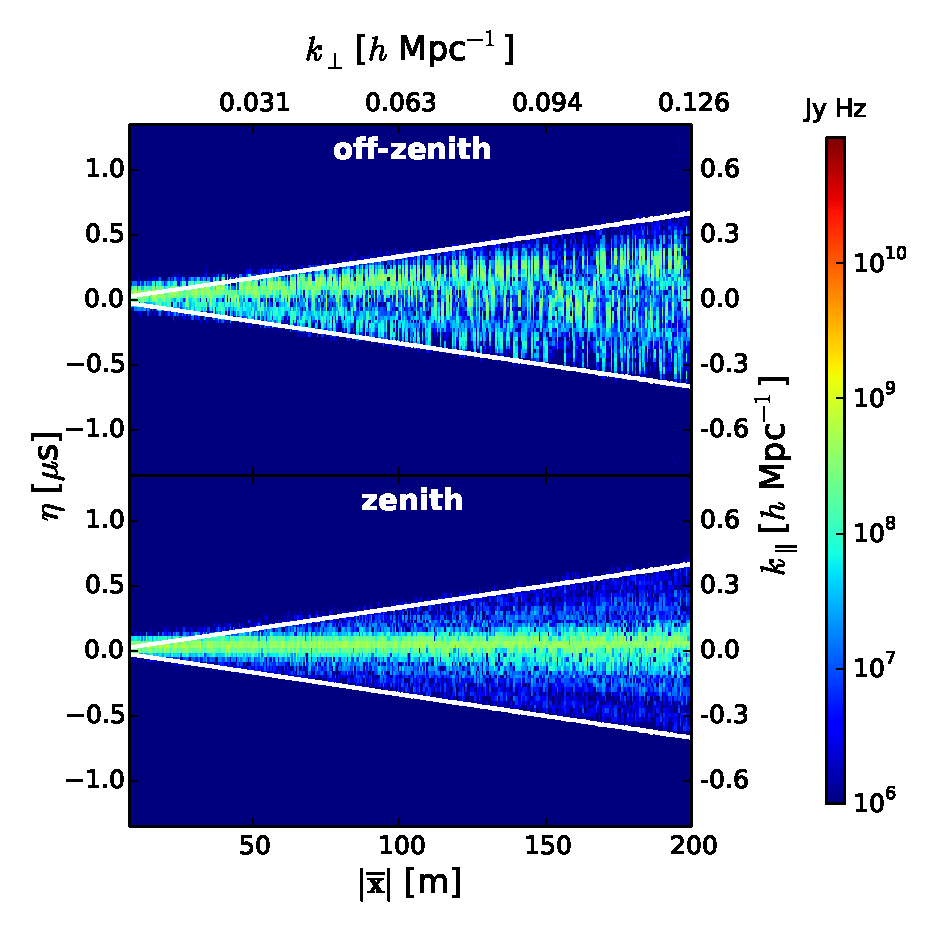
\includegraphics[width=\linewidth]{figures/v1_0/delta_array_multi_baseline_CLEAN_noiseless_visibilities_0.3m_ground_custom_gaussian_FG_model_csm_all_sky_nside_64_Tsys_95.0K_185.0_MHz_30.7_MHz_bhw2.0.eps}
\caption{Same as Figure~\ref{fig:noiseless-dsm-delay-spectrum} but for a foreground model consisting of compact emission. Compact emission gives rise to centrally concentrated features and stays flat across antenna spacings in the {\it foreground wedge}.\label{fig:noiseless-csm-delay-spectrum}}
\end{figure}

The amplitude response of an interferometer to a point source is, to first order, flat with respect to baseline length. Since the main lobe of the power--pattern in the {\it off--zenith} pointing is centered eastward of zenith, the bulk of the compact foreground emission is seen in a branch with positive delay corresponding to the position of the primary lobe of the power--pattern. In the {\it zenith} pointing, compact emission from the same patch of sky is seen as a bright horizontal arm at zero delay  since the primary lobe of the power--pattern is centered at zenith. 

Foreground emission in zero delay and negative delay regions in the {\it off--zenith} pointing is caused by point sources co--located with secondary lobes of the power--pattern. On the other hand, point sources co--located with secondary lobes of power--pattern in the {\it zenith} pointing are revealed as faint but distinct branches at positive and negative delays depending on the orientation of antenna spacing and direction of emission on the sky. 

\subsection{The ``Pitchfork''}\label{sec:composite}

Delay spectra from the all--sky foreground model in our study display a composite feature set drawn from the features of compact and diffuse foreground models. Here we compare the relative strengths of emission from different spatial scales in our all--sky composite foreground model. 

When not dominated by the bright emission from the Galactic center, which happens only for certain pointings at certain times, the delay spectrum of the combined foreground model is composed of diffuse and compact emission, in roughly equal measure. This is illustrated by a more detailed examination of the {\it zenith} pointing in our study. 

Figure~\ref{fig:pitchfork-baselines} shows delay spectra of three antenna pairs of different antenna spacings oriented northward during the {\it zenith} pointing; each is a different vertical slice of the two dimensional delay spectrum plots shown in Figures~\ref{fig:fhd_data}, \ref{fig:sim_data}, \ref{fig:noiseless-dsm-delay-spectrum}, and \ref{fig:noiseless-csm-delay-spectrum}. The diffuse, compact, and composite components are shown as solid red, cyan, and black lines, respectively. The horizon delay limits are shown as a pair of vertical dotted lines. The gray shaded area denotes the envelope of expected uncertainty in the delay spectrum. Uncertainty in emission in the {\it foreground} wedge (between the horizon delay limits) is dominated by the $\gtrsim$~70\% error owing to uncertainties in predicting the spectral index of compact foreground model, while thermal noise fluctuations dominate outside. 

\begin{figure}[htb]
\centering
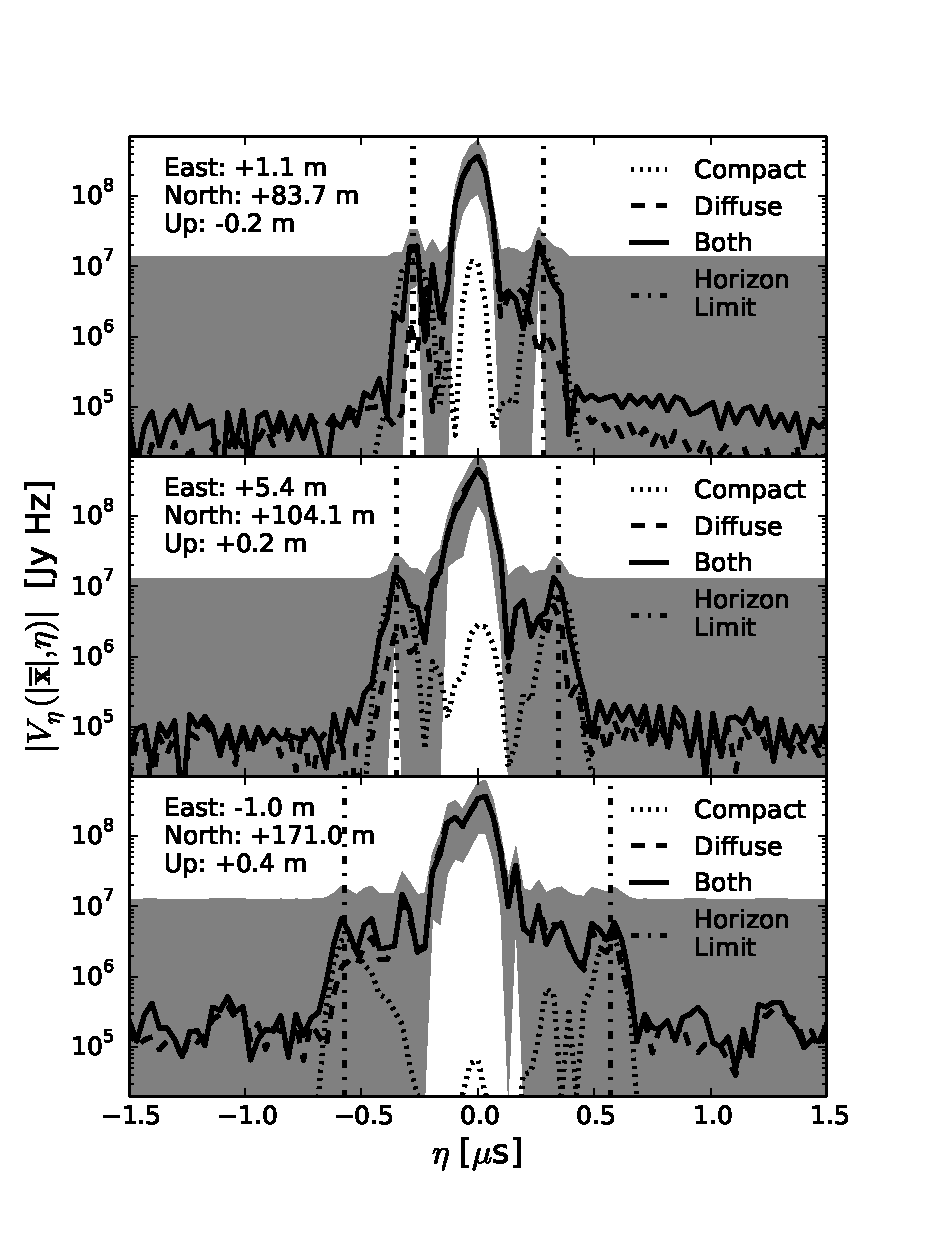
\includegraphics[width=\linewidth]{figures/v1_0/delta_array_3_baseline_comparison_CLEAN_noiseless_visibilities_0.3m_ground_custom_gaussian_FG_model_all_sky_nside_64_Tsys_95.0K_185.0_MHz_30.7_MHz_bhw2.0.eps}
\caption{Simulated delay spectrum amplitudes $|V_{b\tau}(\vec{b},\tau)|$ for three chosen northward oriented antenna spacings of length: $\sim$84~m ({\it top}), $\sim$104~m ({\it middle}), and $\sim$171~m ({\it bottom}). The antenna spacing is specified in each panel along East, North and Upward directions. The solid red, cyan, and black lines denote contributions from diffuse, compact, and composite foreground models respectively. Vertical dotted lines mark the horizon delay limits. The shaded region denotes the envelope of uncertainty around the composite model delay spectrum. This uncertainty is dictated by uncertainties in spectral indices of foreground models inside the delay horizon delay limits. Outside the horizon delay limits, it is predominantly due to thermal noise fluctuations. Compact emission dominates the central regions of delay spectrum while both components, especially diffuse emission on short antenna spacings, dominate near the horizon delay limits, giving rise to a {\it pitchfork}--shaped structure. \label{fig:pitchfork-baselines}}
\end{figure}

The zero--delay peak (corresponding to the main lobe in the power--pattern) with a value of $\sim 10^8$--$10^9$~Jy~Hz, independent of antenna spacing, is predominantly determined by compact emission. The corresponding peak at zero--delay from diffuse foreground model is at least 10 times fainter and decreases drastically with an increase in antenna spacing. This is the response expected from different antenna spacings towards compact and diffuse emission. 

Near the horizon delay limits at shorter antenna spacing, the diffuse component is brighter relative to the compact component. Here, diffuse emission does not decrease as rapidly with increasing antenna spacing as was seen at zero--delay. In fact, even on widely spaced antennas, {\emph diffuse emission in the delay spectrum near the horizon delay limits exceeds that in the main lobe by more than two orders of magnitude}. We attribute this to apparent shortening of antenna spacings projected in the direction of diffuse emission entering far from the primary field of view, thereby giving rise to the edge--heavy {\it two--pronged fork} feature discussed in \S\ref{sec:diffuse-long-baselines}.

Simulations with the complete foreground model show the combination of center--heavy features on all antenna spacings from compact emission, and edge--heavy features from both compact and diffuse emission especially the latter even on wide antenna spacings.  This results in a characteristic {\it pitchfork} structure imprinted in the {\it foreground} wedge and should be evident in observations.

All these observations are consistent with those from Figures~\ref{fig:noiseless-dsm-delay-spectrum} and \ref{fig:noiseless-csm-delay-spectrum}. The observability of the {\it pitchfork} signature predicted in this paper depends on the relative levels of uncertainty in the foreground model and fluctuations from thermal noise. In our simulations, since thermal noise in these very short duration snapshots is $\gtrsim 10^7$~Jy~Hz, and features near the horizon delay limits are $\sim 10^7$~Jy~Hz, the {\it pitchfork} feature is not expected to be detected in a noisy scenario although this feature is marginally visible in the {\it zenith} pointing of observed data (see Figure~\ref{fig:fhd_data}). We attribute this to differences between our foreground model and the actual sky.  Deeper observations should reveal the feature clearly.

We also note that increasing the antenna spacing results in progressively improving the resolution along the delay axis by increasing the number of delay bins inside the {\it foreground wedge}. This improves the localization of foreground objects whose signatures are imprinted in the delay spectrum. For instance, there is an increase in the number of secondary peaks in the delay spectrum between zero--delay and horizon delay limits as the antenna spacing increases from $\sim$84~m to $\sim$170~m. In this case, these correspond to secondary lobes of the power--pattern that lie between the primary lobe and the horizon along the local meridian. At short antenna spacings, due to relatively lower resolution along the delay axis inside the {\it foreground wedge} and a consequent loss of localization of foreground emission, these secondary peaks blend in with other major peaks and are not distinctly visible. These findings are consistent with the discussion in \S\ref{sec:compact}.

In summary, the brightest signature ($\gtrsim 10^{10}$~Jy~Hz) is that of the Galactic center in the {\it off--zenith} pointing co--located at a westward secondary lobe with a significantly high gain. The next brightest signature ($\sim 10^8$--$10^9$~Jy~Hz) is caused by compact emission appearing to be concentrated in the inner regions of the {\it foreground wedge} (near zero delays) rather than towards the boundaries. Diffuse emission co--located at the primary lobe of the power--pattern is fainter by approximately an order of magnitude relative to compact emission from the same region for a $\sim 84$~m antenna spacing. But unlike the latter, diffuse emission decreases rapidly by over two orders of magnitude as the antenna spacing is widened to $\sim 170$~m. However, diffuse emission is significantly higher near horizon delay limits compared to that in the primary lobe of the power--pattern as the antenna spacing is increased. This leads to edge--heavy features in the delay spectrum. Complemented by the center-heavy compact foreground features, we predict the presence of a {\it three--pronged pitchfork}--shaped signature in the delay spectrum of the foreground sky. We identify evidence for presence of this signature in actual MWA data, although deeper observations are needed to more clearly reveal the effect.

\section{Applications}\label{sec:fg-grading}

% While the {\it foreground wedge} is a region of high foreground contamination, of particular interest to the EoR community is foreground contamination near horizon delay limits. These regions are believed to be responsible for significant spillover into the relatively clean {\it EoR window} due to spectral response of the instrument and foregrounds. 

Here, we will investigate the susceptibility of particular antenna spacings to foreground contamination arising out of bright foreground objects located near the horizon and present a technique to substantially mitigate such contamination.

The Galactic center in the {\it off--zenith} pointing is one such example already available in our study. Figure~\ref{fig:sky-model} shows the sky model ({\it top:} compact component, {\it bottom:} diffuse component) in this pointing. The Galactic center is the most dominant source of foreground contamination from the diffuse sky model and is co--located with a bright secondary lobe of the power pattern near the western horizon. Figure~\ref{fig:delay-map} shows the sky mapped to delays registered by the baseline vectors, of length 100~m for instance, oriented northward (top panel) and eastward (bottom panel). Since the Galactic center is located in the western sky, this figure demonstrates that it is observed at negative delay on a baseline vector oriented eastward and at zero delay on a baseline vector oriented northward. Figure~\ref{fig:baseline-breakup} shows the delay spectra on baselines oriented northward (67\fdg 5~$\le \theta_\textrm{b} <$~112\fdg 5) at the top and eastward (-22\fdg 5~$\le \theta_\textrm{b} <$~22\fdg 5) at the bottom. The Galactic center manifests itself most distinctly near the negative horizon delay limit on short eastward baselines in the delay spectrum (bottom panel of Figure~\ref{fig:baseline-breakup}). Consequently, the spillover caused by the instrument's transfer function from the {\it foreground wedge} into the {\it EoR window} affects the northward baselines the least and is most severe in eastward baselines (particularly the short ones) evident by the bright vertical stripes of foreground contamination. 

\begin{figure*}[htb]
\centering
\subfloat[][Sky model]{\label{fig:sky-model}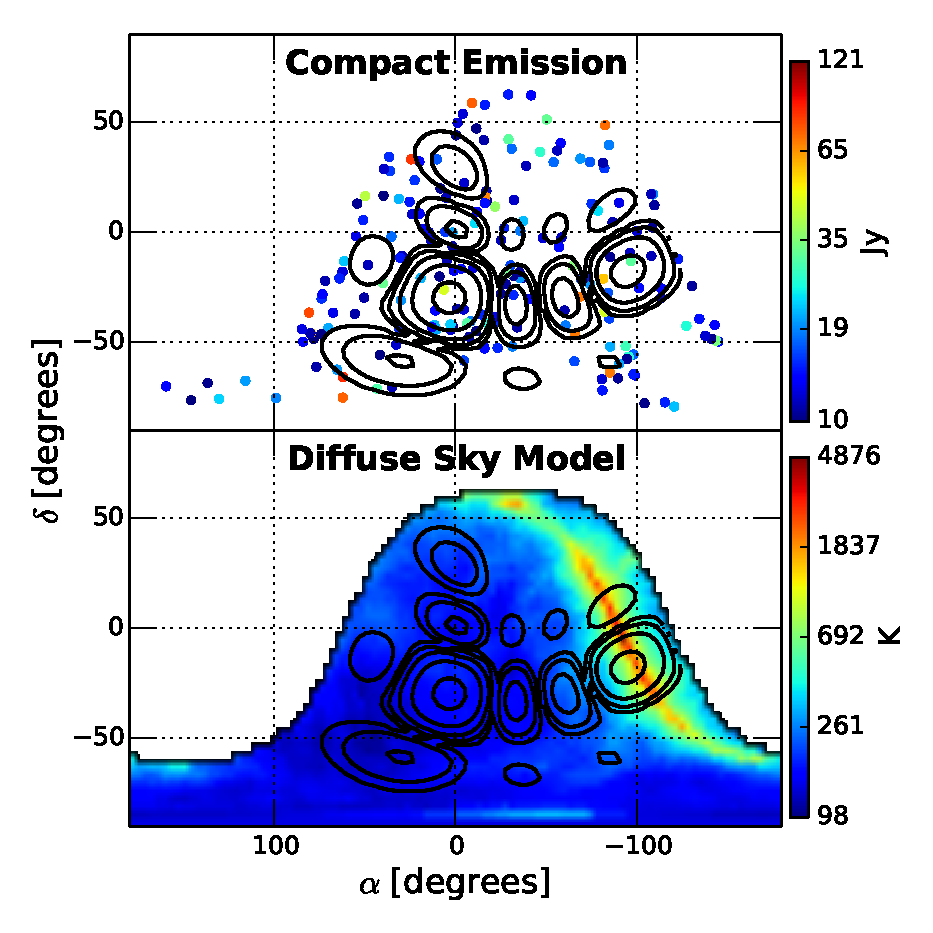
\includegraphics[width=0.33\linewidth]{figures/v1_0/sky_model_snapshot_0.eps}}
\subfloat[][Delay maps]{\label{fig:delay-map}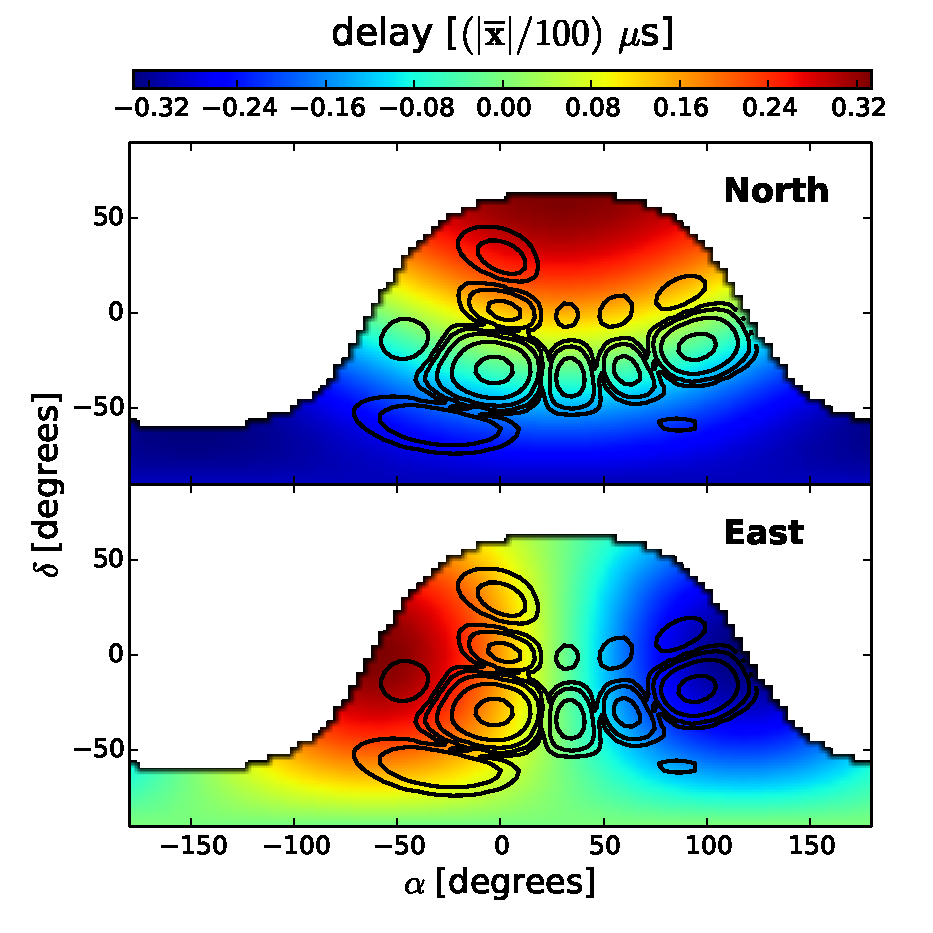
\includegraphics[width=0.33\linewidth]{figures/v1_0/directional_delay_map_snapshot_0.eps}}
\subfloat[][Delay Spectra]{\label{fig:baseline-breakup}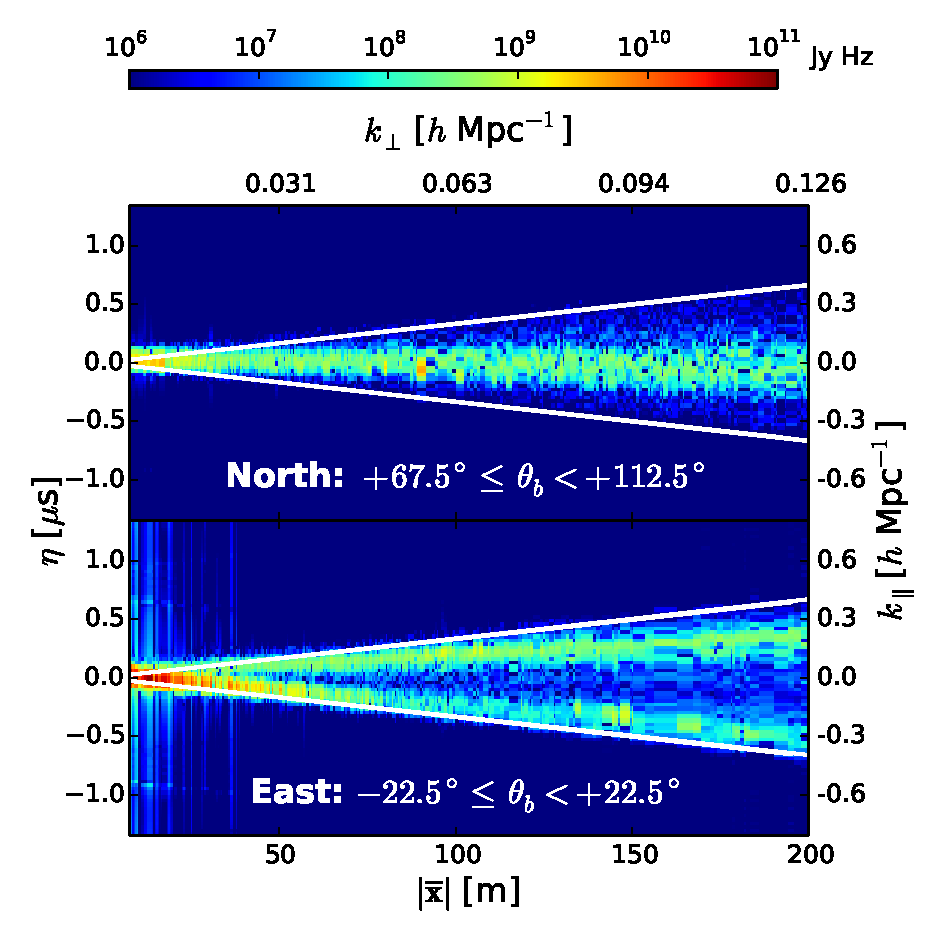
\includegraphics[width=0.33\linewidth]{figures/v1_0/baseline_orientation_breakup_snapshot_0.eps}}
\caption{(a): Sky model showing compact ({\it top}) and diffuse ({\it bottom}) emission. Contours of power pattern are overlaid whose levels are identical to those in Figures~\ref{fig:DSM} and \ref{fig:CSM}. The Galactic center is very prominent in diffuse emission in the western sky and is co--located with a bright secondary lobe of the power pattern. (b): Sky hemisphere mapped to delays observed on antenna spacings with northward ({\it top}) and eastward ({\it bottom}) orientations. Color scale shown is for a 100~m antenna spacing. Delays vary linearly with antenna spacing length. The bright Galactic center in the western sky is recorded at zero delays in northward antenna spacings and close to negative horizon delay limit on eastward antenna spacings. (c): Simulated delay spectra $|V_{b\tau}(\vec{b},\tau)|$ on antenna spacings oriented northward ({\it top}) and eastward ({\it bottom}). White lines denote horizon delay limits. The bright Galactic center is prominently visible close to negative horizon delay limit, especially on short eastward antenna spacings. These are also the most severely contaminated by foreground spillover. The northward antenna spacings, on the other hand, are the least contaminated.}
\label{fig:breakup}
\end{figure*}

The delay spectrum, $V_{b\tau}(\vec{b},\tau)$, not only carries information on spatial scales of foreground emission but also offers the unique advantage of viewing the sky through a combination of antenna spacing vectors and the delay axis. With a foreground model known {\it a priori} in which structures and locations of very bright foreground objects such as the Galactic center or AGN are available, we can predict their response across antenna spacings as a function of observing parameters such as LST, power--pattern, etc. This allows us to programmatically screen data for antenna spacings that are severely contaminated by foregrounds near the horizon delay limits in the delay spectrum. These can be weighted appropriately during data analysis. We demonstrate such a screening technique, whereby we use the bright object's location and structure to discard antenna spacings of certain lengths and orientations to mitigate foreground contamination in the {\it EoR window}. 

In our example, we discard eastward antenna spacings (-22\fdg 5~$\le\theta_\textrm{b}<$~22\fdg 5) of lengths $|\vec{b}| < 30$~m. Figure~\ref{fig:before-after} shows the delay spectra obtained with all antenna spacings (top panel) and after applying our screening technique (bottom panel) on the {\it off--zenith} observation. Notice the remarkable reduction in foreground spillover into the {\it EoR window} via the removal of bright vertical stripes on short eastward antenna spacings. The color scale range has been adjusted relative to the previous figures to show this significant reduction in foreground contamination. 

\begin{figure}[htb]
\centering
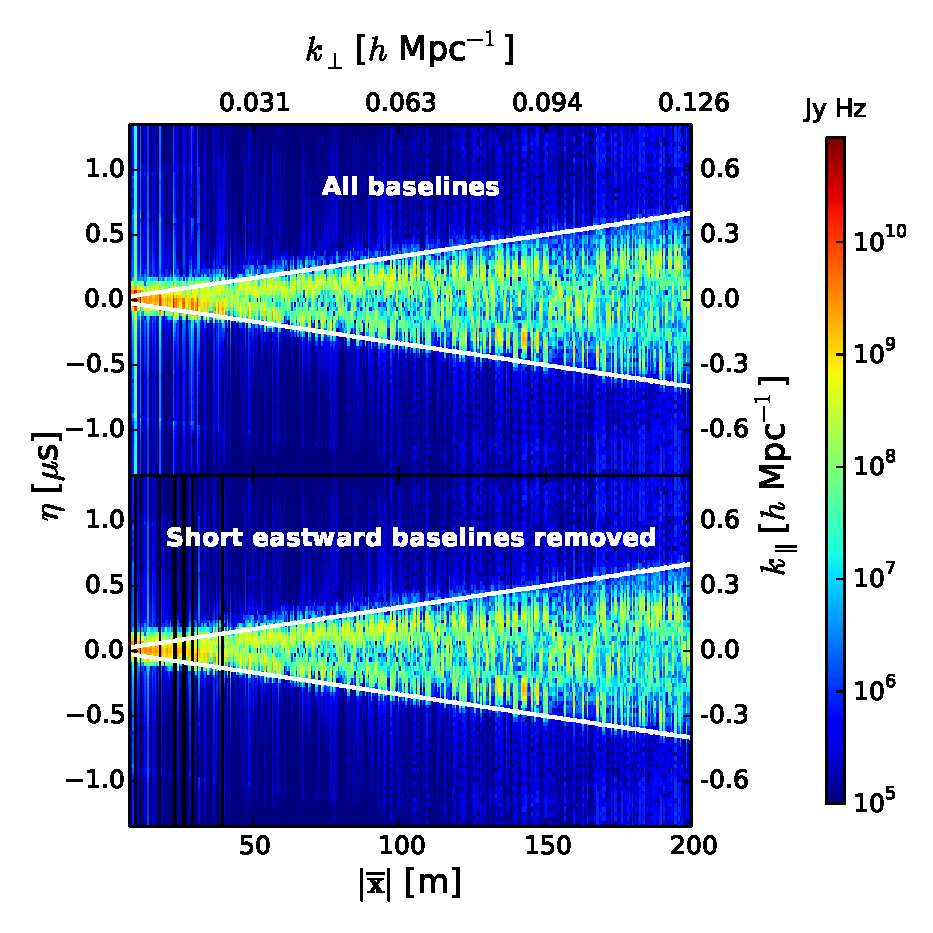
\includegraphics[width=\linewidth]{figures/v1_0/baseline_screening_before_after_nside_64_Tsys_95.0K.eps}
\caption{Simulated delay spectra amplitudes $|V_{b\tau}(\vec{b},\tau)|$ for the {\it off--zenith} pointing with all antenna spacings included ({\it top}) and with short eastward antenna spacings discarded ({\it bottom}). Discarded antenna spacings (black vertical stripes) have lengths $|\vec{b}|<30$~m (leftward of vertical dashed line) and orientations $|\theta_\textrm{b}|<$~22\fdg 5. The spillover from the bright Galactic center near the negative horizon delay limit from the {\it foreground wedge} prominent when all antenna spacings are used is lowered by an order of magnitude when short eastward antenna spacings are discarded. Color scale has been adjusted to emphasize mitigation achieved in foreground contamination. \label{fig:before-after}}
\end{figure}

This screening technique can be generalized to optimize between foreground mitigation and loss of sensitivity from discarding data. Figure~\ref{fig:screening} shows how the typical foreground contamination\footnote{We use standard deviation of noiseless $V_{b\tau}(\vec{b},\tau)$ from foregrounds in the {\it EoR window} as a measure of foreground contamination.} in the {\it EoR window} depends on the orientations and lengths of discarded antenna spacings. We choose antenna spacings oriented eastward to varying degrees of directedness, i.e., -7\fdg 5~$\le\theta_\textrm{b}<$~7\fdg 5 (solid circles), -15\arcdeg~$\le\theta_\textrm{b}<$~15\arcdeg~ (solid squares), and -22\fdg 5~$\le\theta_\textrm{b}<$~22\fdg 5 (solid stars). Among antenna spacings that satisfy these criteria, we discard data from those whose lengths are shorter than $|\vec{b}|_\textrm{max}$ ($x$--axis) and show foreground contamination estimated in the {\it EoR window} from all remaining antenna spacings. In other words, these plots demonstrate the progress in mitigation as orientation and maximum length of discarded antenna spacings are varied. % Foreground contamination estimated from only northward (dashed line) and eastward (dot--dashed line) antenna spacings represent the lower and upper limits, respectively, and are shown for reference. 
The fraction of discarded antenna spacings discarded relative to the total number is shown in dotted lines for different ranges of $\theta_\textrm{b}$. It is seen that foreground contamination can be mitigated by a factor between $\sim 1.5$ ($|\theta_\textrm{b}|\le$~7\fdg 5) and $\sim 10$ ($|\theta_\textrm{b}|\le$~22\fdg 5). It is notable that short antenna spacings play maximum role in determining foreground contamination. For instance, among antenna spacings with orientations $|\theta_\textrm{b}|\le$~22\fdg 5, discarding those with lengths $|\vec{b}|\gtrsim 30$~m does not mitigate foreground contamination any further and would only lead to loss of sensitivity as the fraction of discarded baselines increases from $\sim 5$\% to $\sim 25$\%. On the other hand, a bright point source at the same location will give rise to foreground contamination even on longer antenna spacings. Such cases will necessitate discarding more or, in the worst case, all of the eastward oriented antenna spacings accounting for $\sim 25$\% loss of data.

\begin{figure}[htb]
\centering
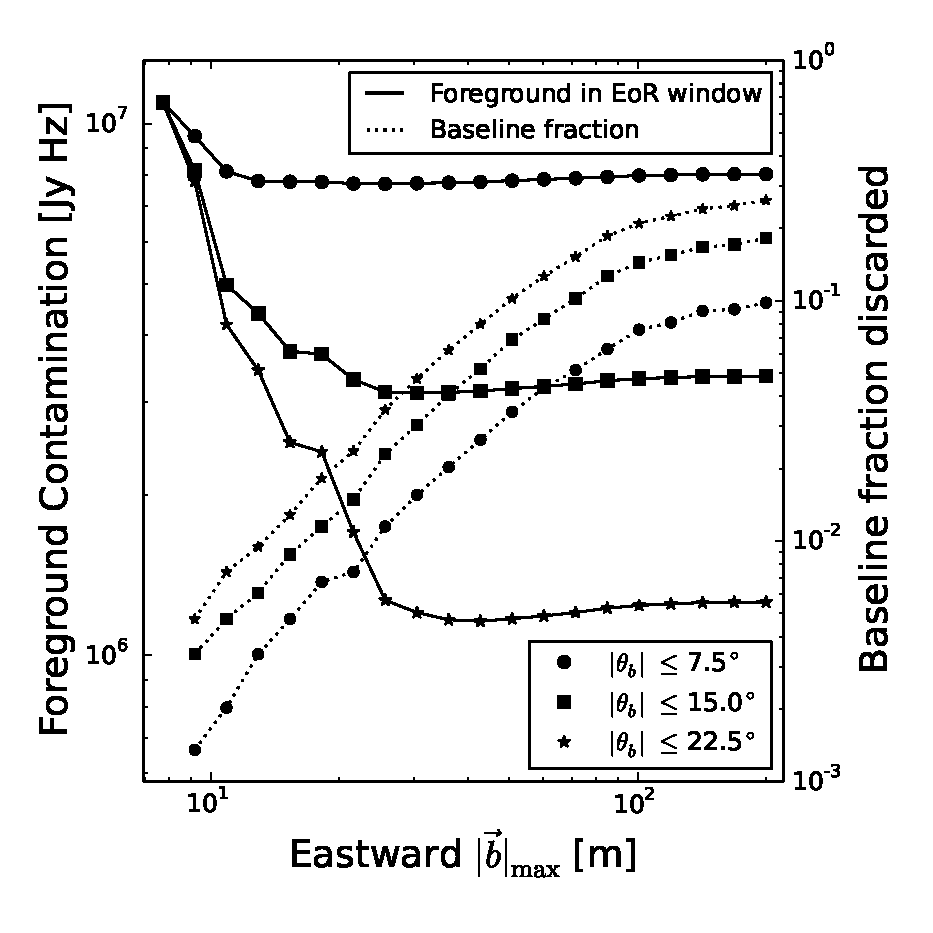
\includegraphics[width=\linewidth]{figures/v1_0/baseline_screening_nside_64_Tsys_95.0K.eps}
\caption{Foreground contamination, estimated using standard deviation in the {\it EoR window}, for the {\it off--zenith} pointing as a function of orientation and length of discarded antenna spacings. Antenna spacings oriented eastward with varying degrees of directedness are considered: -7\fdg 5~$\le\theta_\textrm{b}<$~7\fdg 5 (solid circles), -15\arcdeg~$\le\theta_\textrm{b}<$~15\arcdeg~ (solid squares), and -22\fdg 5~$\le\theta_\textrm{b}<$~22\fdg 5 (solid stars). Among antenna spacings that satisfy the above criteria, ones with lengths $\le |\vec{b}|_\textrm{max}$ ($x$--axis) are discarded. The fraction of discarded antenna spacings relative to the total number is denoted by dotted lines for the corresponding cases. % Lower (dashed line) and upper (dot--dashed) limits on foreground contamination are derived from northward (67\fdg 5~$\le\theta_\textrm{b}<$~112\fdg 5) and eastward ($|\theta_\textrm{b}|\le$~22\fdg 5) antenna spacings respectively. 
  Foreground contamination in the {\it EoR window} (solid lines) reduces by factor $\sim$1.5 ($|\theta_\textrm{b}|\le$~7\fdg 5) to $\sim$10 ($|\theta_\textrm{b}|\le$~22\fdg 5). Short baselines have maximum effect on foreground contamination. For instance, discarding antenna spacings oriented $|\theta_\textrm{b}|\le$~22\fdg 5 with lengths $|\vec{b}|\gtrsim 30$~m has no effect in further reducing foreground contamination. \label{fig:screening}}
\end{figure}

In principle, instead of discarding selected antenna spacings altogether, we could down--weight them based on an optimal scheme. This technique provides a very simple and yet effective tool in adding a layer of control to mitigate effects of foreground contamination in EoR data analysis. % The success behind clear identification of severely foreground--contaminated antenna pairs based on delay spectrum technique depends on the localization of the source of foreground contamination and its strength. 

\section{Summary}\label{sec:summary}

Our primary motivation in this work is to understand how the various bright foregrounds will manifest in three dimensional power spectrum of H{\sc i} from 21~cm reionization observations. When the signal is expressed in units of temperature variance, the dynamic range between bright foregrounds and the 21~cm signal is expected to be $\sim 10^8$; a detailed understanding of how foregrounds can corrupt the 21~cm power spectrum is therefore essential. This analysis extends previous work by simulating the entire sky rather than just the central field of view and by providing a comparison with early observations from the MWA. By making use of the delay spectrum technique to estimate the power spectrum, we are able to observe the effects of foregrounds while avoiding entanglements with more complex power spectrum estimators.  

Simulating in all important respects the response of the MWA to an all--sky foreground model that consists of diffuse Galactic emission from \citet{deo08} and bright point sources from the NVSS and SUMSS catalogs, we confirm that the modeled delay spectra are in agreement with data obtained with the MWA, to the extent allowed by levels of uncertainty known in the foreground models and thermal noise fluctuations in measurements. 

Our simulations enable us to identify numerous signatures of different components of foreground emission seen in the delay spectra. We establish the relationship between these signatures and observing parameters such as antenna pointing and LST, instrument parameters such as antenna power--pattern, and foreground parameters such as the nature of emission, spectral index, etc. 

The bright Galactic center at the edge of the western horizon co--located with one of the far secondary lobes of MWA tile power--pattern is the brightest source of foreground contamination in the {\it off--zenith} pointing. It manifests itself near the negative horizon delay limit in the delay spectrum on antenna spacings oriented eastward. 

As expected, diffuse emission in the primary beam of the antenna power--pattern is prominent on shorter antenna spacings. However, the most interesting result is its footprint on wide antenna spacings near the horizon delay limits, an edge--heavy {\it two--pronged fork}--shaped signature. This is due to apparent shortening of wide antenna spacings in the direction of foreground emission far off--axis, thereby retaining their response to extended emission. On the other hand, compact emission predominantly maps onto central regions of the {\it foreground wedge}. Features arising from compact emission co--located with primary and secondary lobes of the antenna power--pattern have been identified. In general, delay spectrum signatures of compact emission are center--heavy, in clear contrast to those from diffuse emission. A composite all--sky foreground model consisting of diffuse and compact foregrounds combines the characteristic individual shapes into a {\it pitchfork}--shaped structure in the {\it foreground wedge}. This will be distinctly visible when the thermal noise floor is sufficiently lowered, as longer observations are processed through the MWA analysis pipelines.

In conclusion, we find that inclusion of emission models, both diffuse and compact, all the way to the horizon is essential to explaining the observed power spectrum. We also provide a simple and effective tool based on the delay spectrum technique to mitigate foreground contamination by an order of magnitude in EoR data analysis by discarding or down--weighting antenna pairs most affected by foreground contamination as a function of antenna spacing vector and time of observation, without significant loss of data.

\acknowledgments

This work was supported by the U. S. National Science Foundation (NSF) through award AST--1109257. DCJ is supported by an NSF Astronomy and Astrophysics Postdoctoral Fellowship under award AST--1401708.  This work makes use of the Murchison Radio-astronomy Observatory, operated by CSIRO. We acknowledge the Wajarri Yamatji people as the traditional owners of the Observatory site. Support for the MWA comes from the NSF (awards: AST-0457585, PHY-0835713, CAREER-0847753, and AST-0908884), the Australian Research Council (LIEF grants LE0775621 and LE0882938), the U.S. Air Force Office of Scientific Research (grant FA9550-0510247), and the Centre for All-sky Astrophysics (an Australian Research Council Centre of Excellence funded by grant CE110001020). Support is also provided by the Smithsonian Astrophysical Observatory, the MIT School of Science, the Raman Research Institute, the Australian National University, and the Victoria University of Wellington (via grant MED-E1799 from the New Zealand Ministry of Economic Development and an IBM Shared University Research Grant). The Australian Federal government provides additional support via the Commonwealth Scientific and Industrial Research Organisation (CSIRO), National Collaborative Research Infrastructure Strategy, Education Investment Fund, and the Australia India Strategic Research Fund, and Astronomy Australia Limited, under contract to Curtin University. We acknowledge the iVEC Petabyte Data Store, the Initiative in Innovative Computing and the CUDA Center for Excellence sponsored by NVIDIA at Harvard University, and the International Centre for Radio Astronomy Research (ICRAR), a Joint Venture of Curtin University and The University of Western Australia, funded by the Western Australian State government.  

\par\bigskip
\bibliographystyle{apj}
\bibliography{eor}

\end{document}
